%%%%%%%%%%%%%%%%%%%%%%%%%%%%%%%%%%%%%%%%%%%%%%%%%%%%%%%%%%%%%%%%%%%%%%%%%%%%%%%%%%%%%%%%%%%%%%%%%%%%%%
%
%   Filename    : appendix_B.tex
%
%   Description : This file will contain information about your Resource Persons
%                 
%%%%%%%%%%%%%%%%%%%%%%%%%%%%%%%%%%%%%%%%%%%%%%%%%%%%%%%%%%%%%%%%%%%%%%%%%%%%%%%%%%%%%%%%%%%%%%%%%%%%%%

\chapter{PNP Interface}
\label{sec:appendixb}
\begin{figure}[!h]
    \centering
    \begin{subfigure}[c]{1\linewidth}
        \centering
        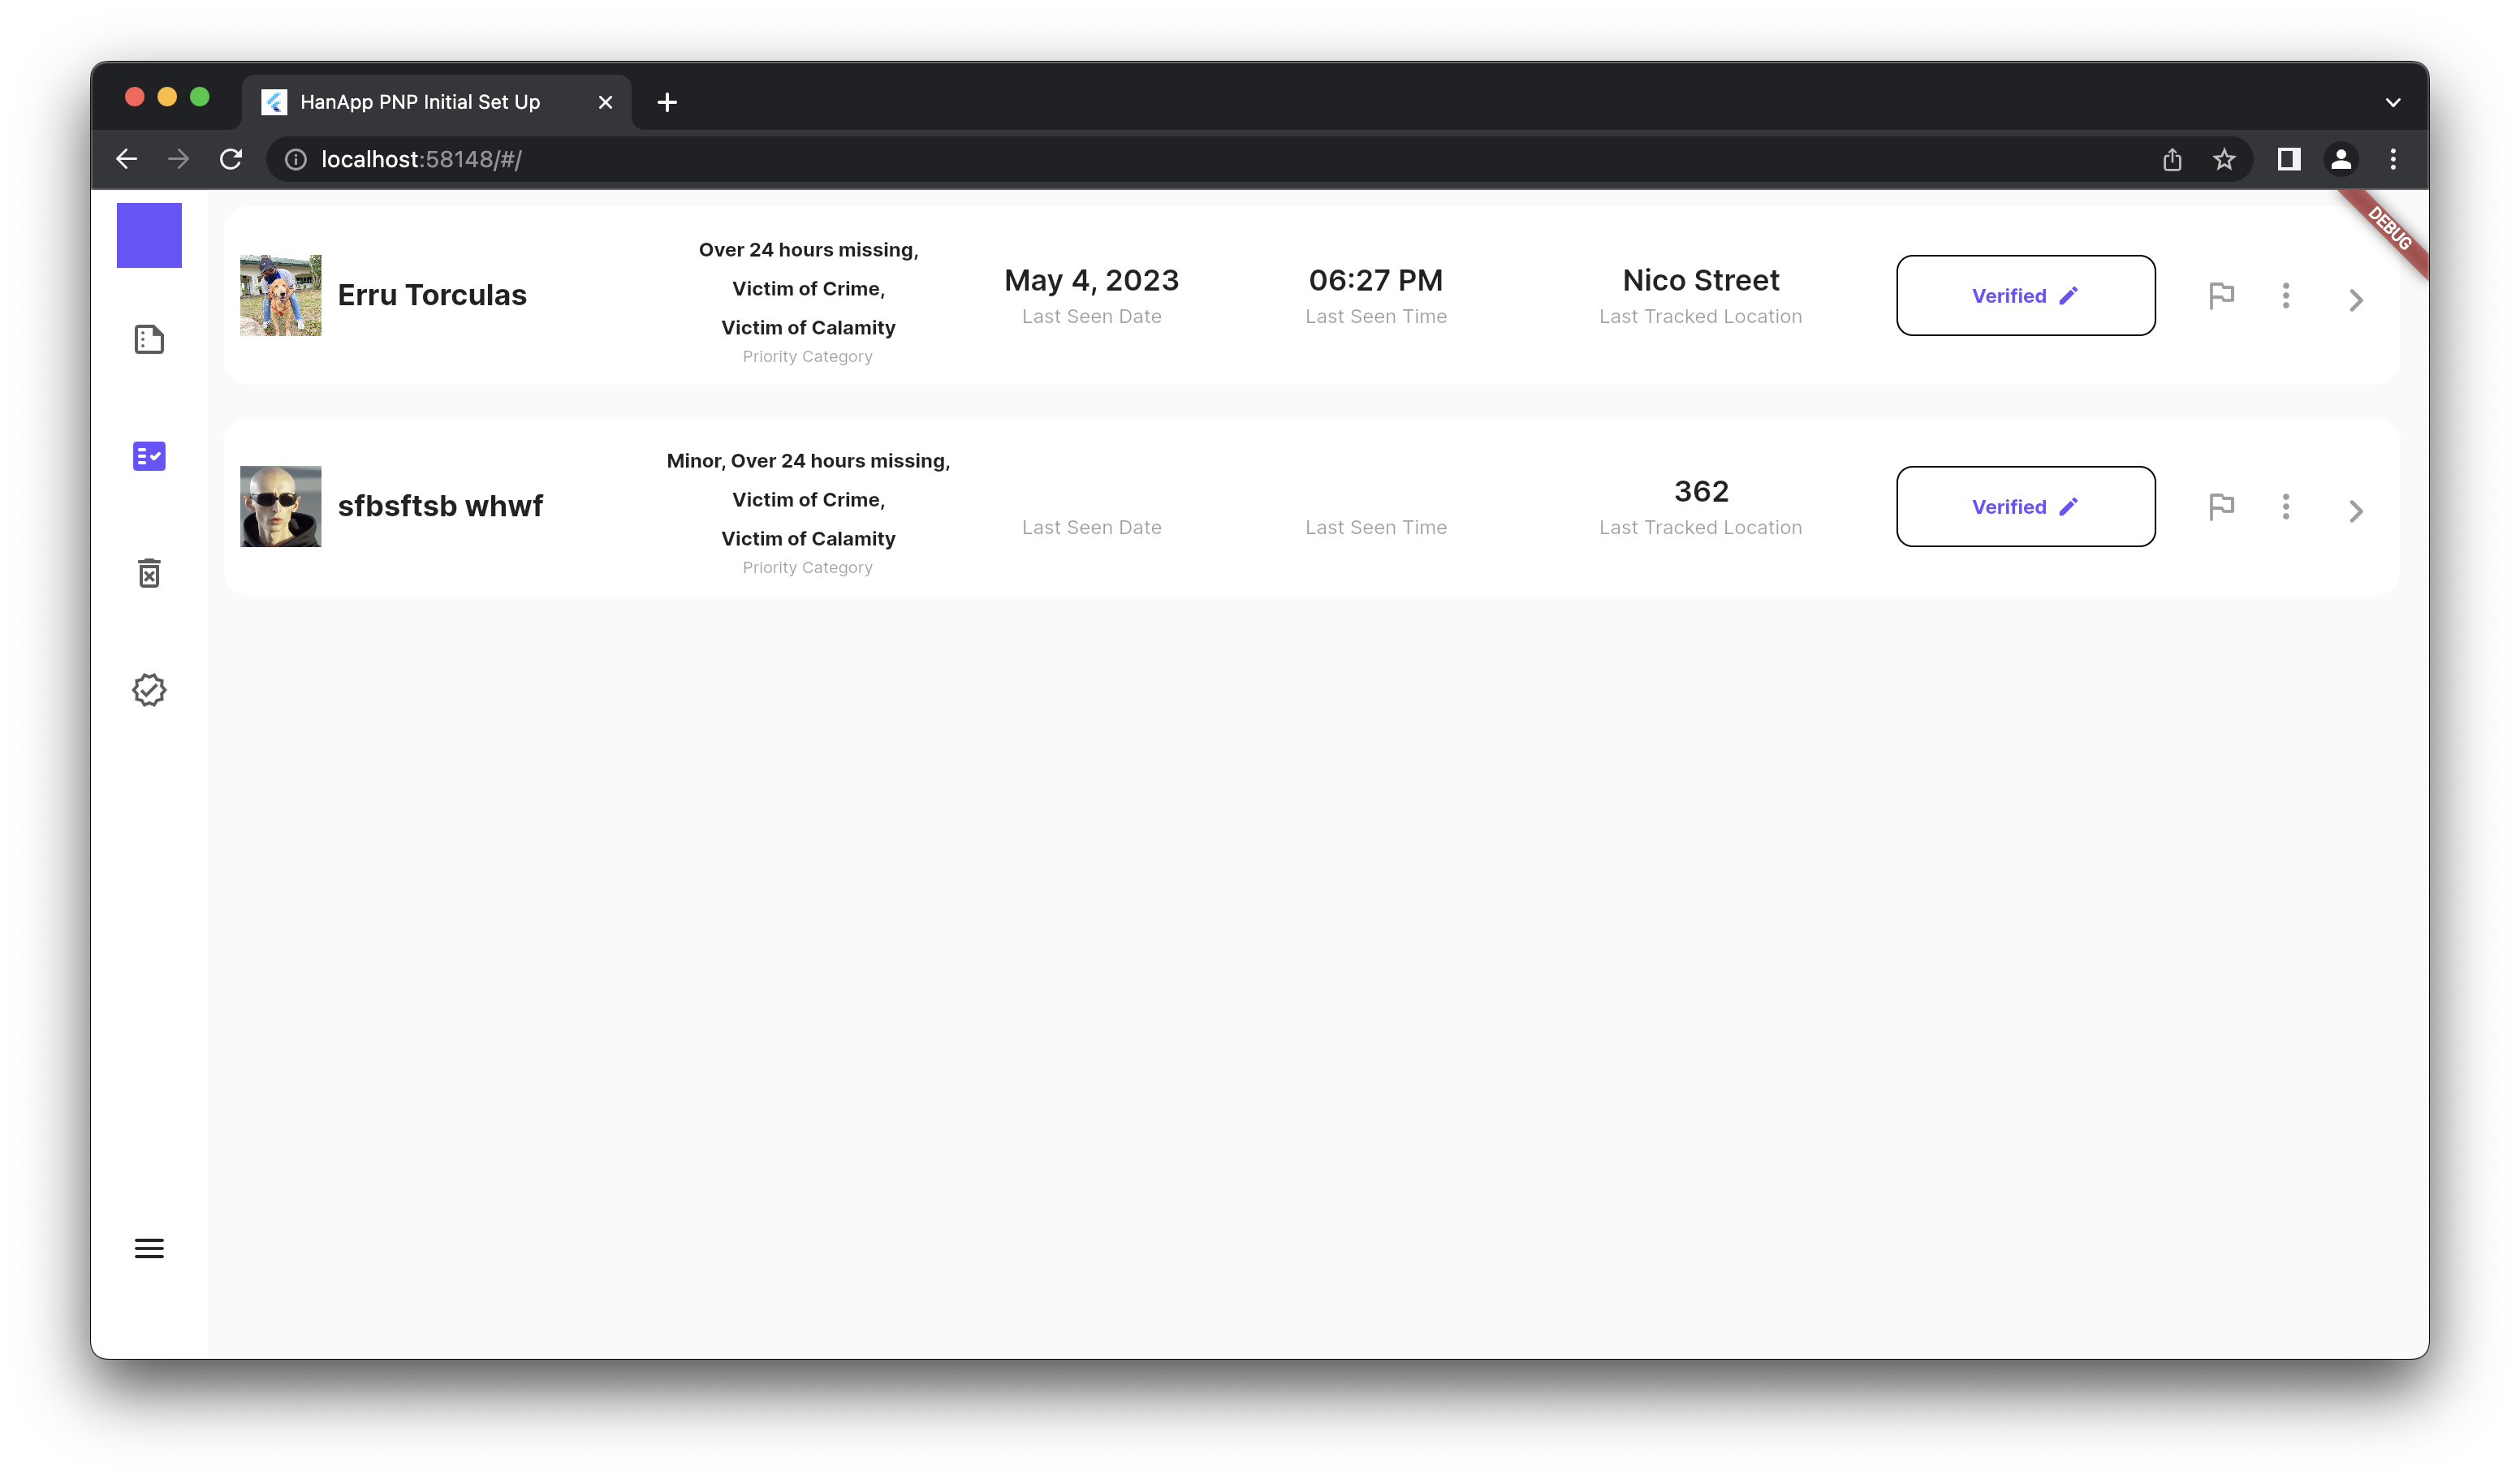
\includegraphics[scale=0.25]{figures/Chapter4/PNP/Verified.png}
    \end{subfigure}
    \caption{Navigation Rail View}
    \label{fig:NavRail}
\end{figure}

\begin{figure}[!h]
    \centering
    \begin{subfigure}[c]{1\linewidth}
        \centering
        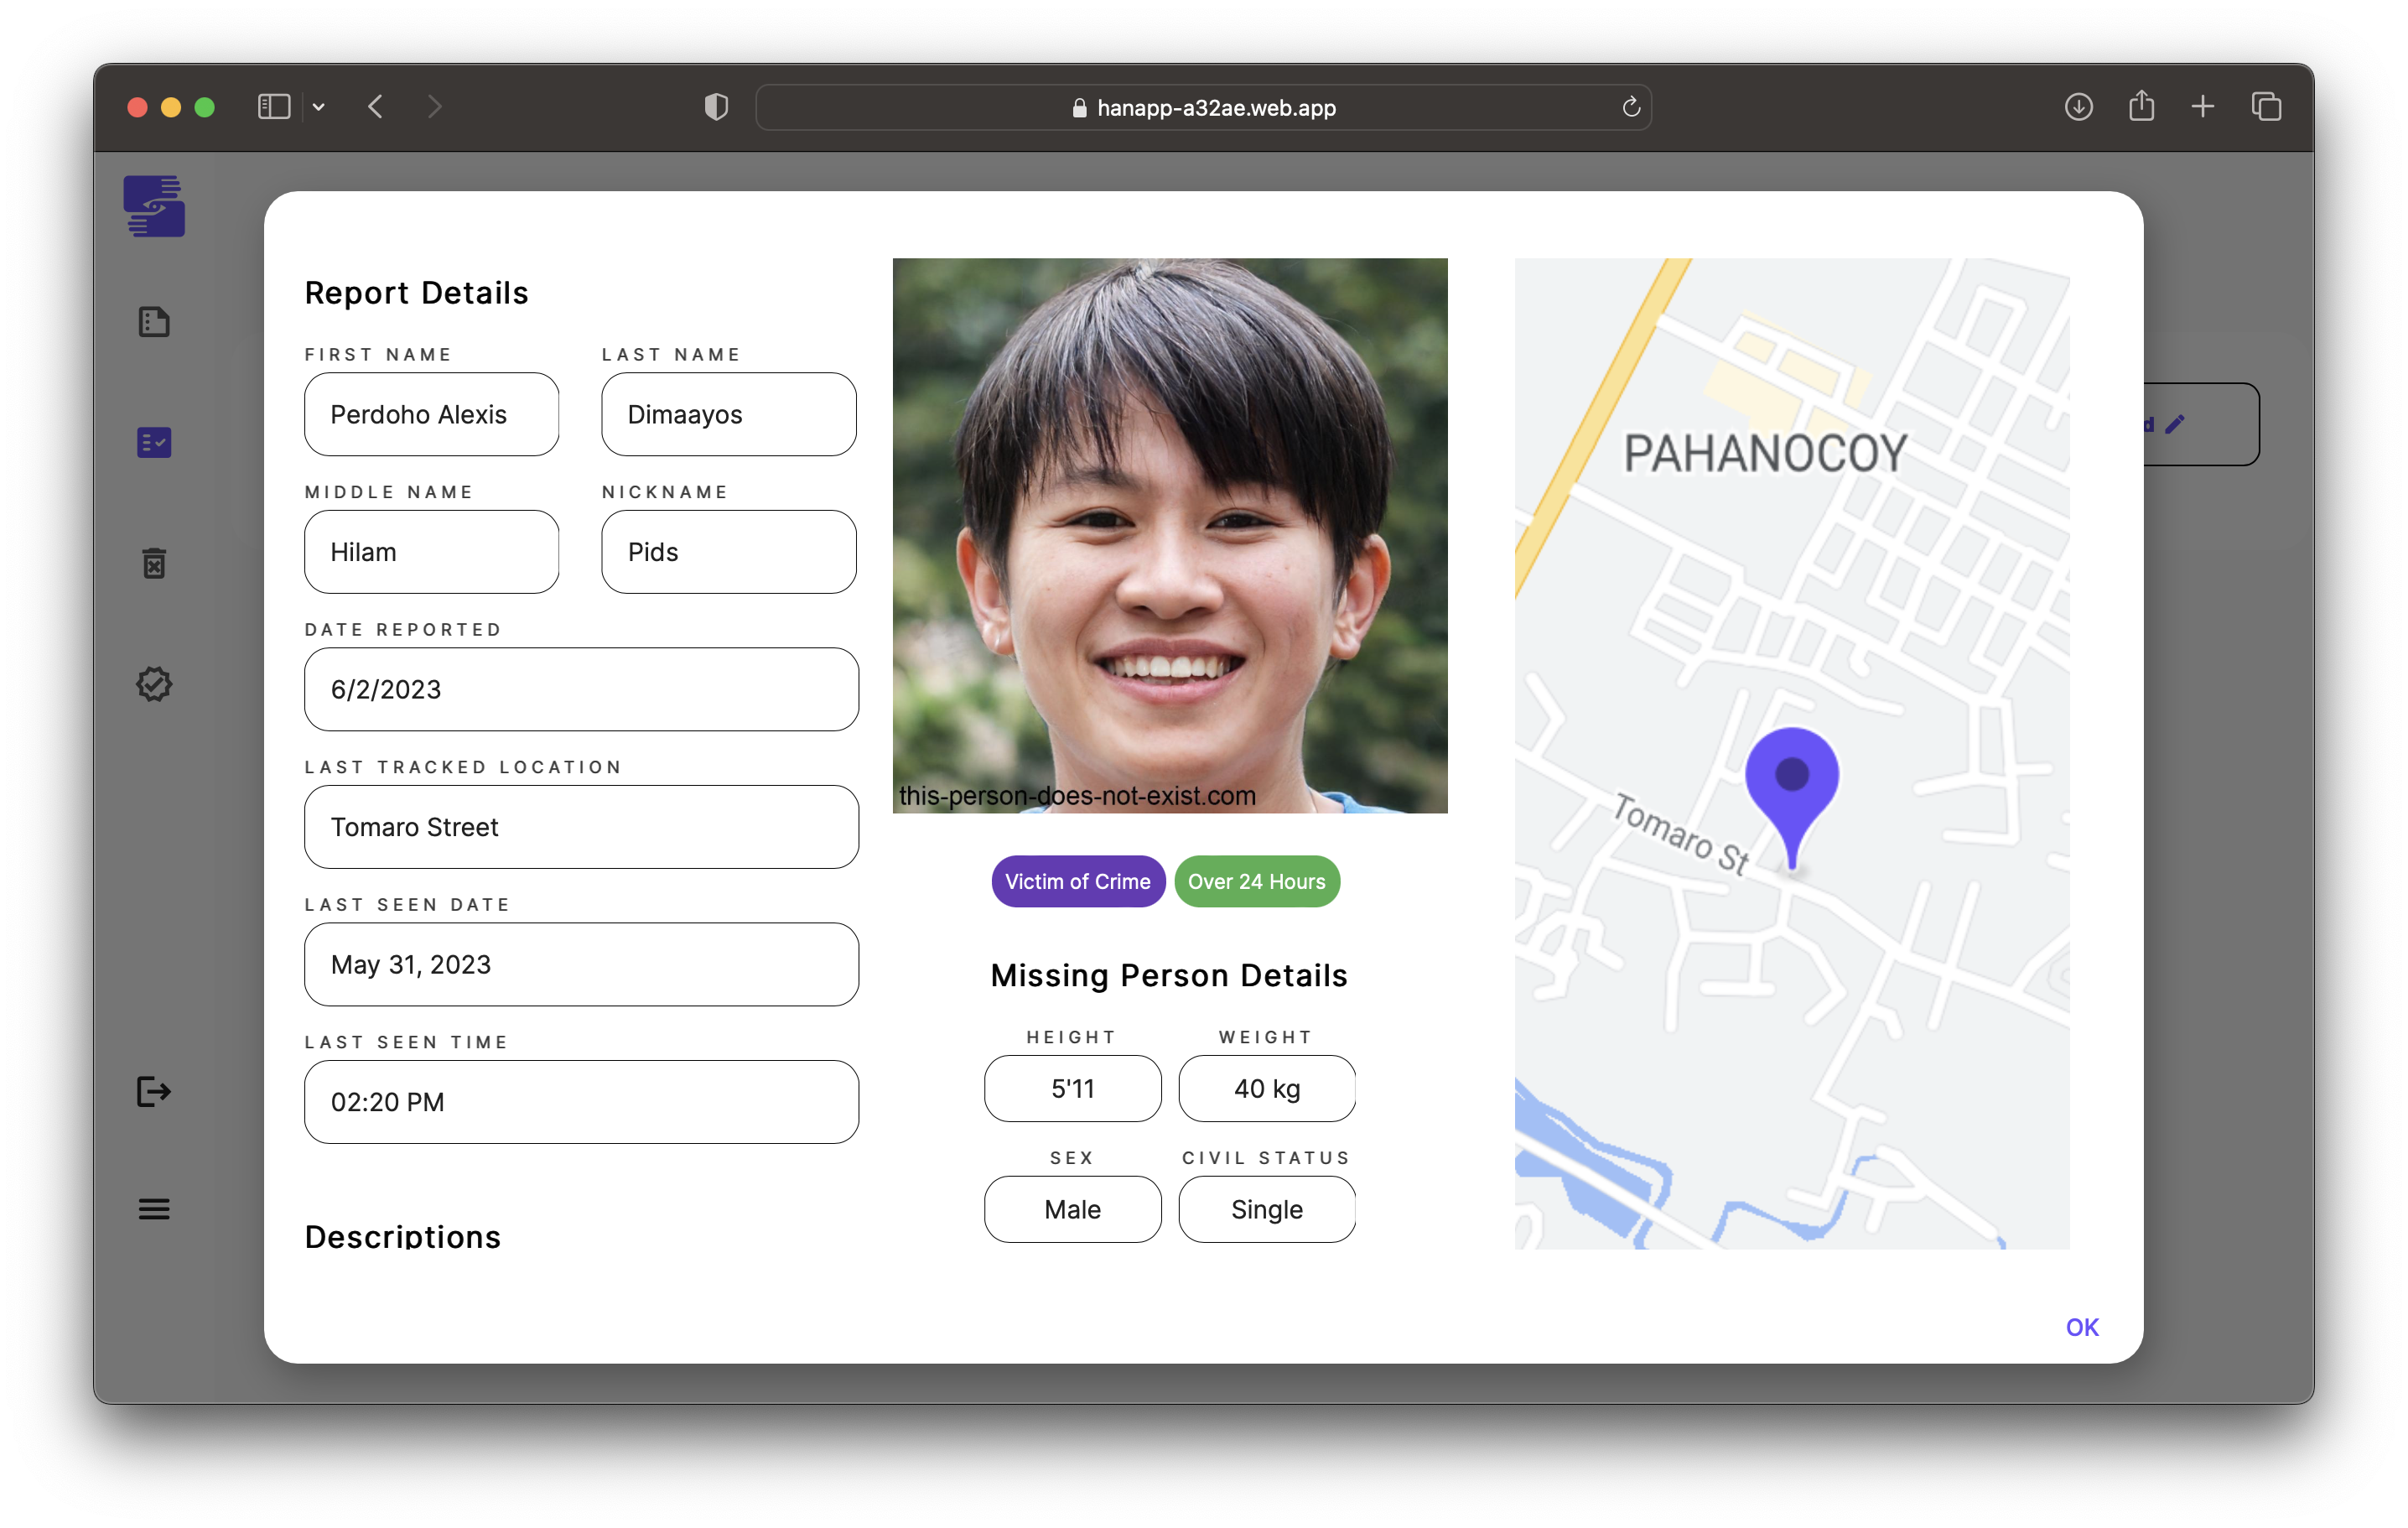
\includegraphics[scale=0.25]{figures/Chapter4/PNP/CaseView-1.png}
    \end{subfigure}
    \centering
    \begin{subfigure}[c]{1\linewidth}
        \centering
        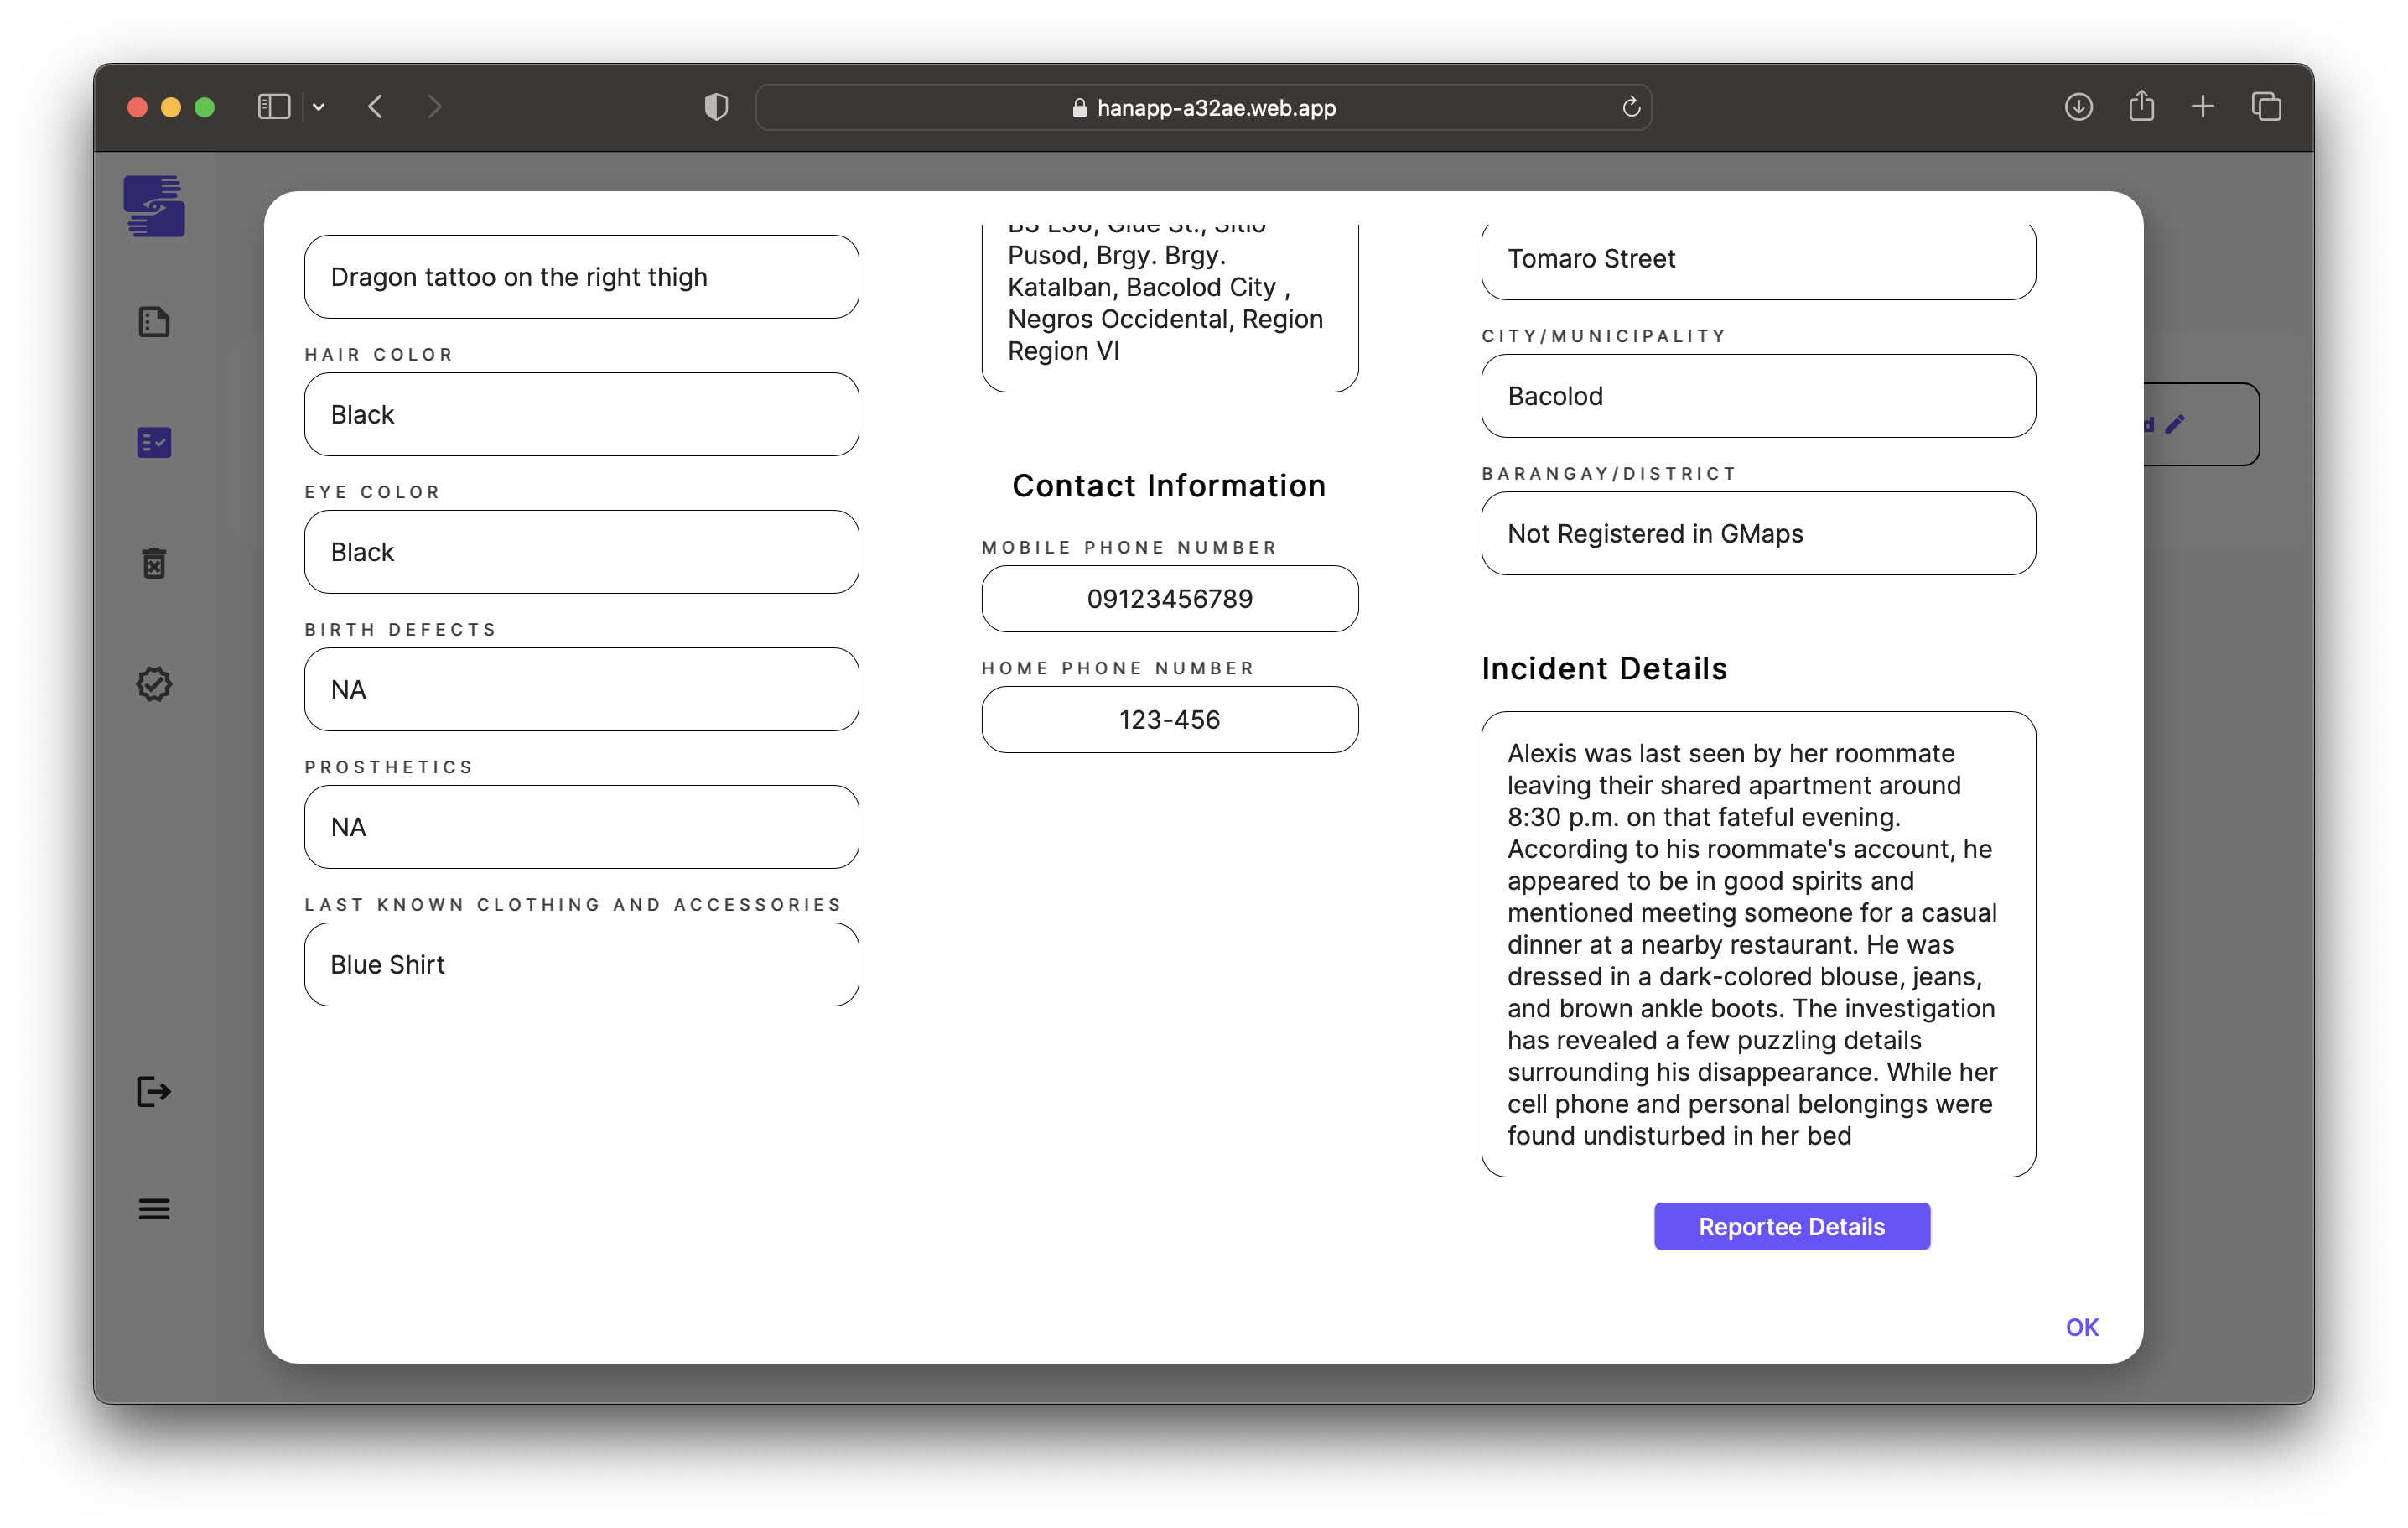
\includegraphics[scale=0.25]{figures/Chapter4/PNP/CaseView-2.png}
    \end{subfigure}
    \caption{Case View of Missing Person}
    \label{fig:caseViewDetails}
\end{figure}

\begin{figure}[!h]
    \centering
    \begin{subfigure}[c]{1\linewidth}
        \centering
        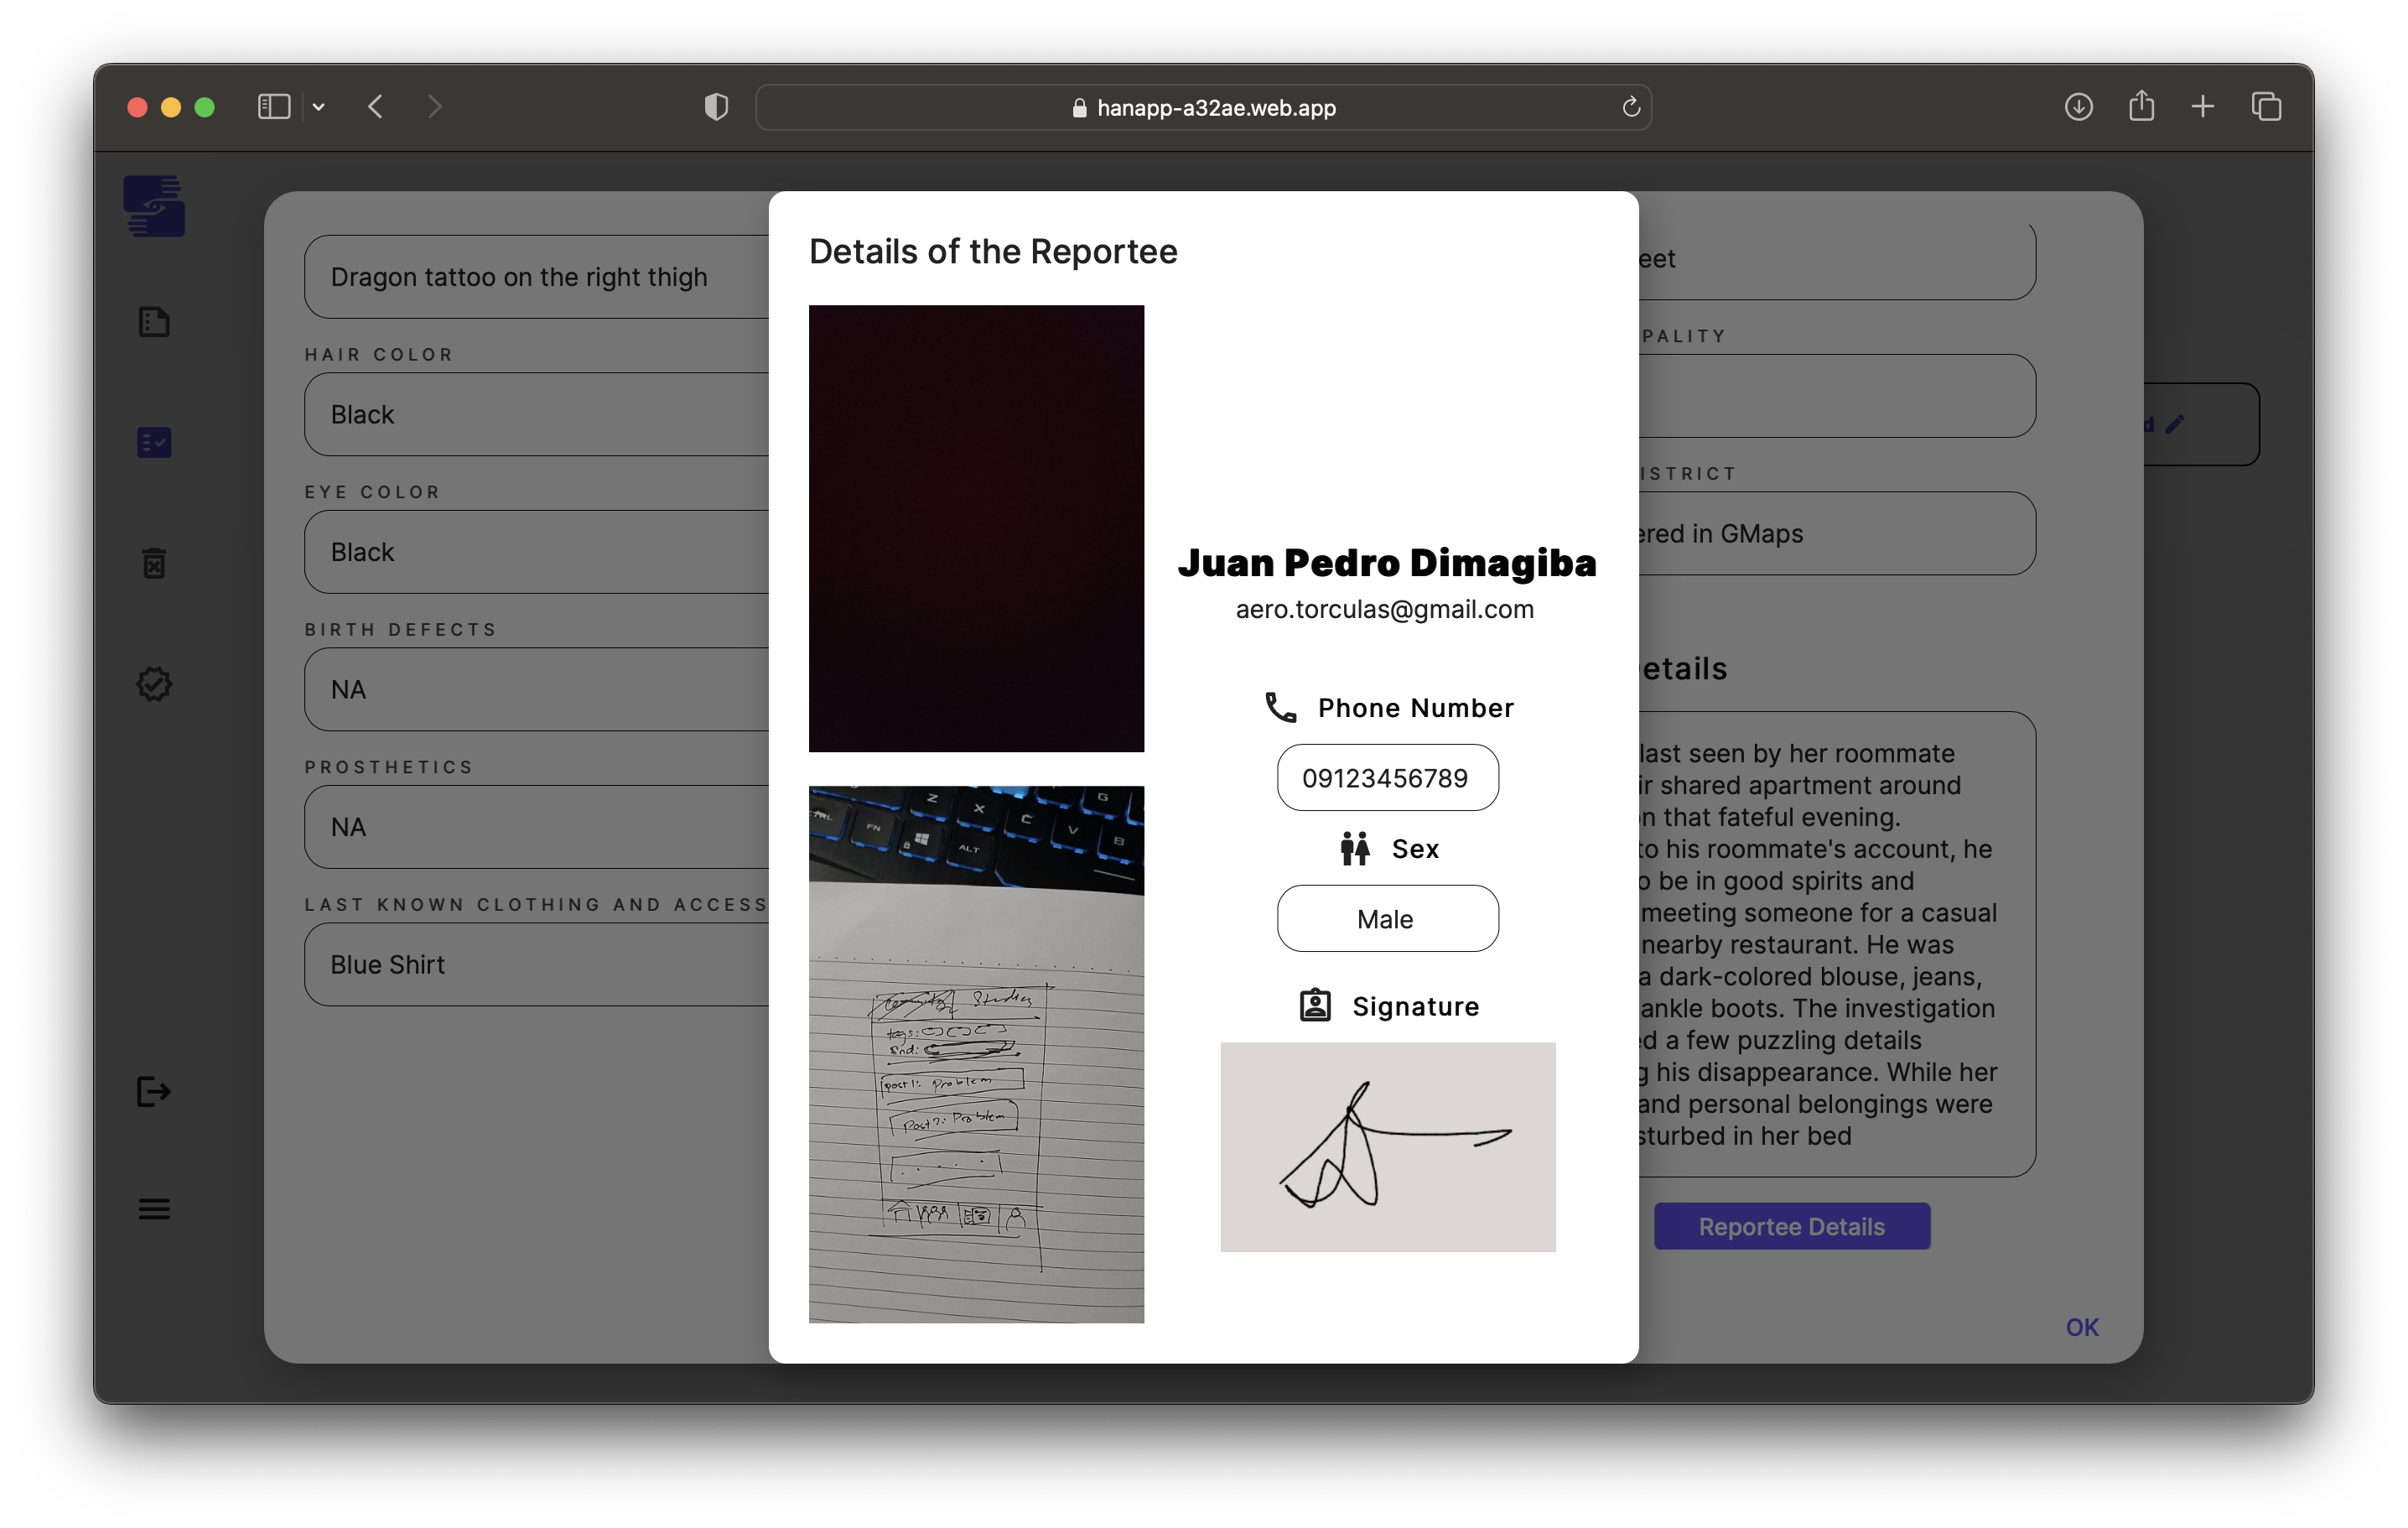
\includegraphics[scale=0.25]{figures/Chapter4/PNP/Reportee.png}
    \end{subfigure}
    \caption{Reportee Details View}
    \label{fig:ReporteeDetails}
\end{figure}

\begin{figure}[!h]
    \centering
    \begin{subfigure}[c]{1\linewidth}
        \centering
        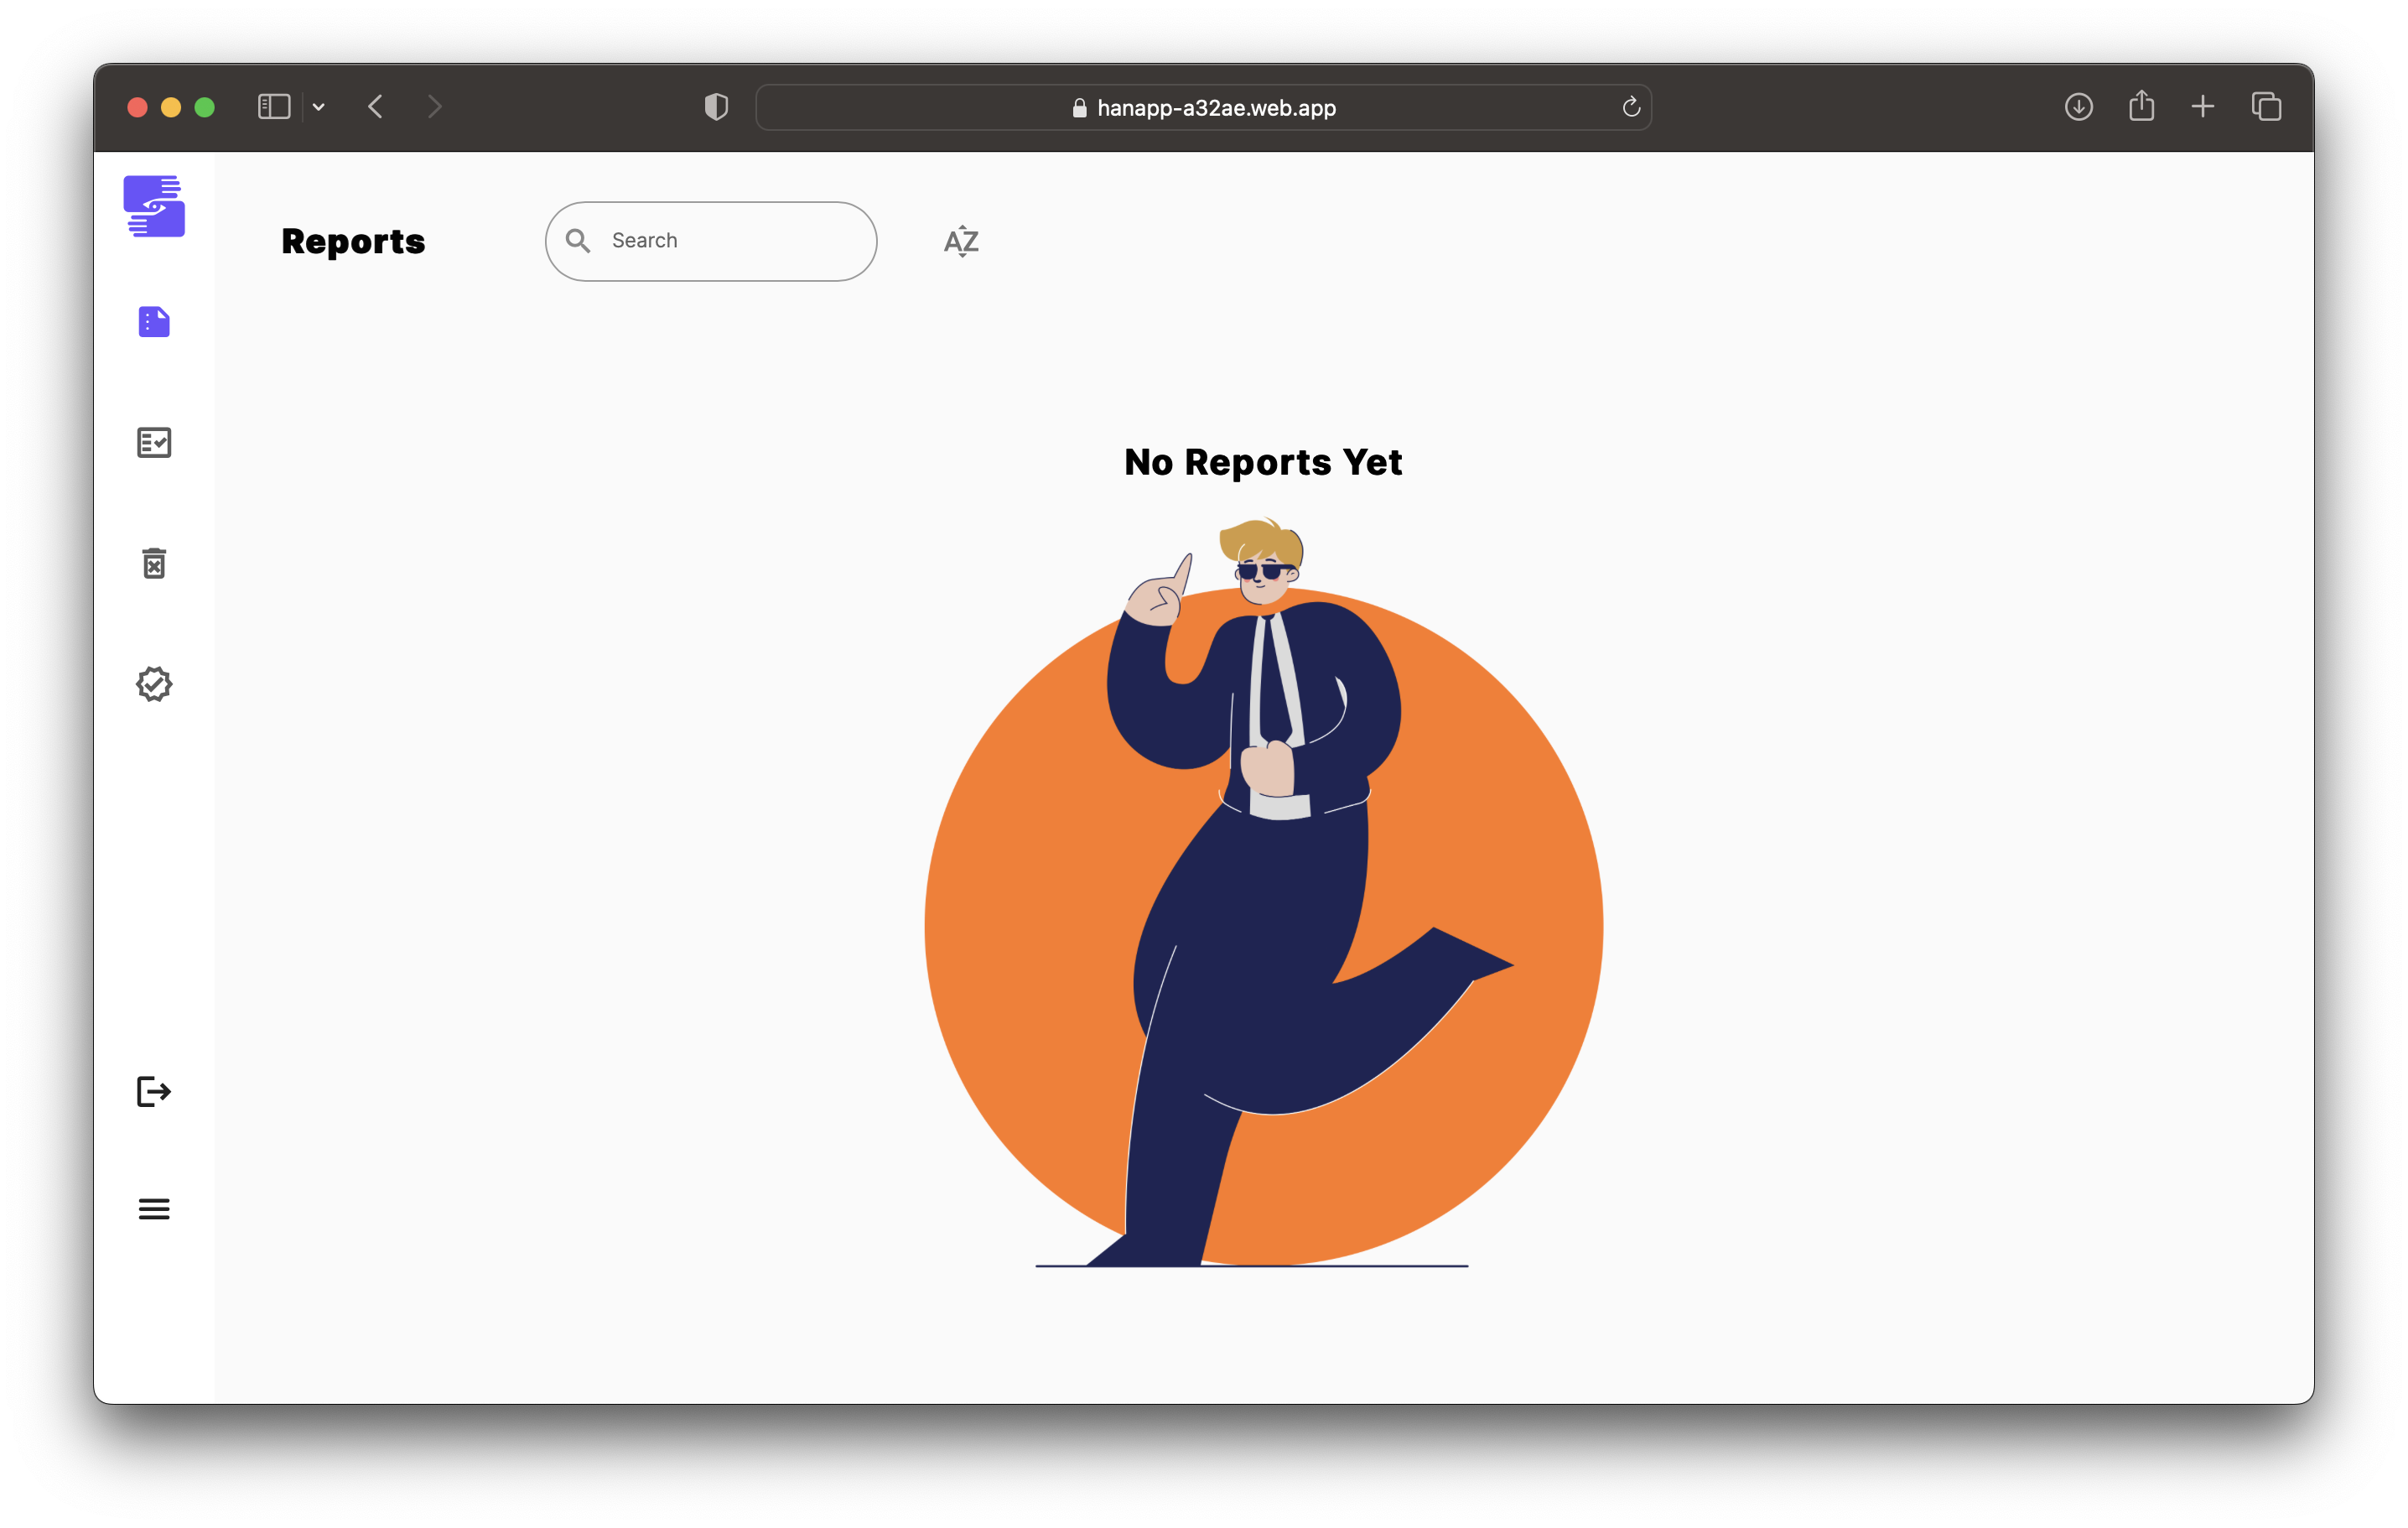
\includegraphics[scale=0.25]{figures/Chapter4/PNP/NoReportsPNP.png}
    \end{subfigure}
    \caption{Empty State of No Reports}
    \label{fig:NoReportsPNP}
\end{figure}

\begin{figure}[!h]
    \centering
    \begin{subfigure}[c]{1\linewidth}
        \centering
        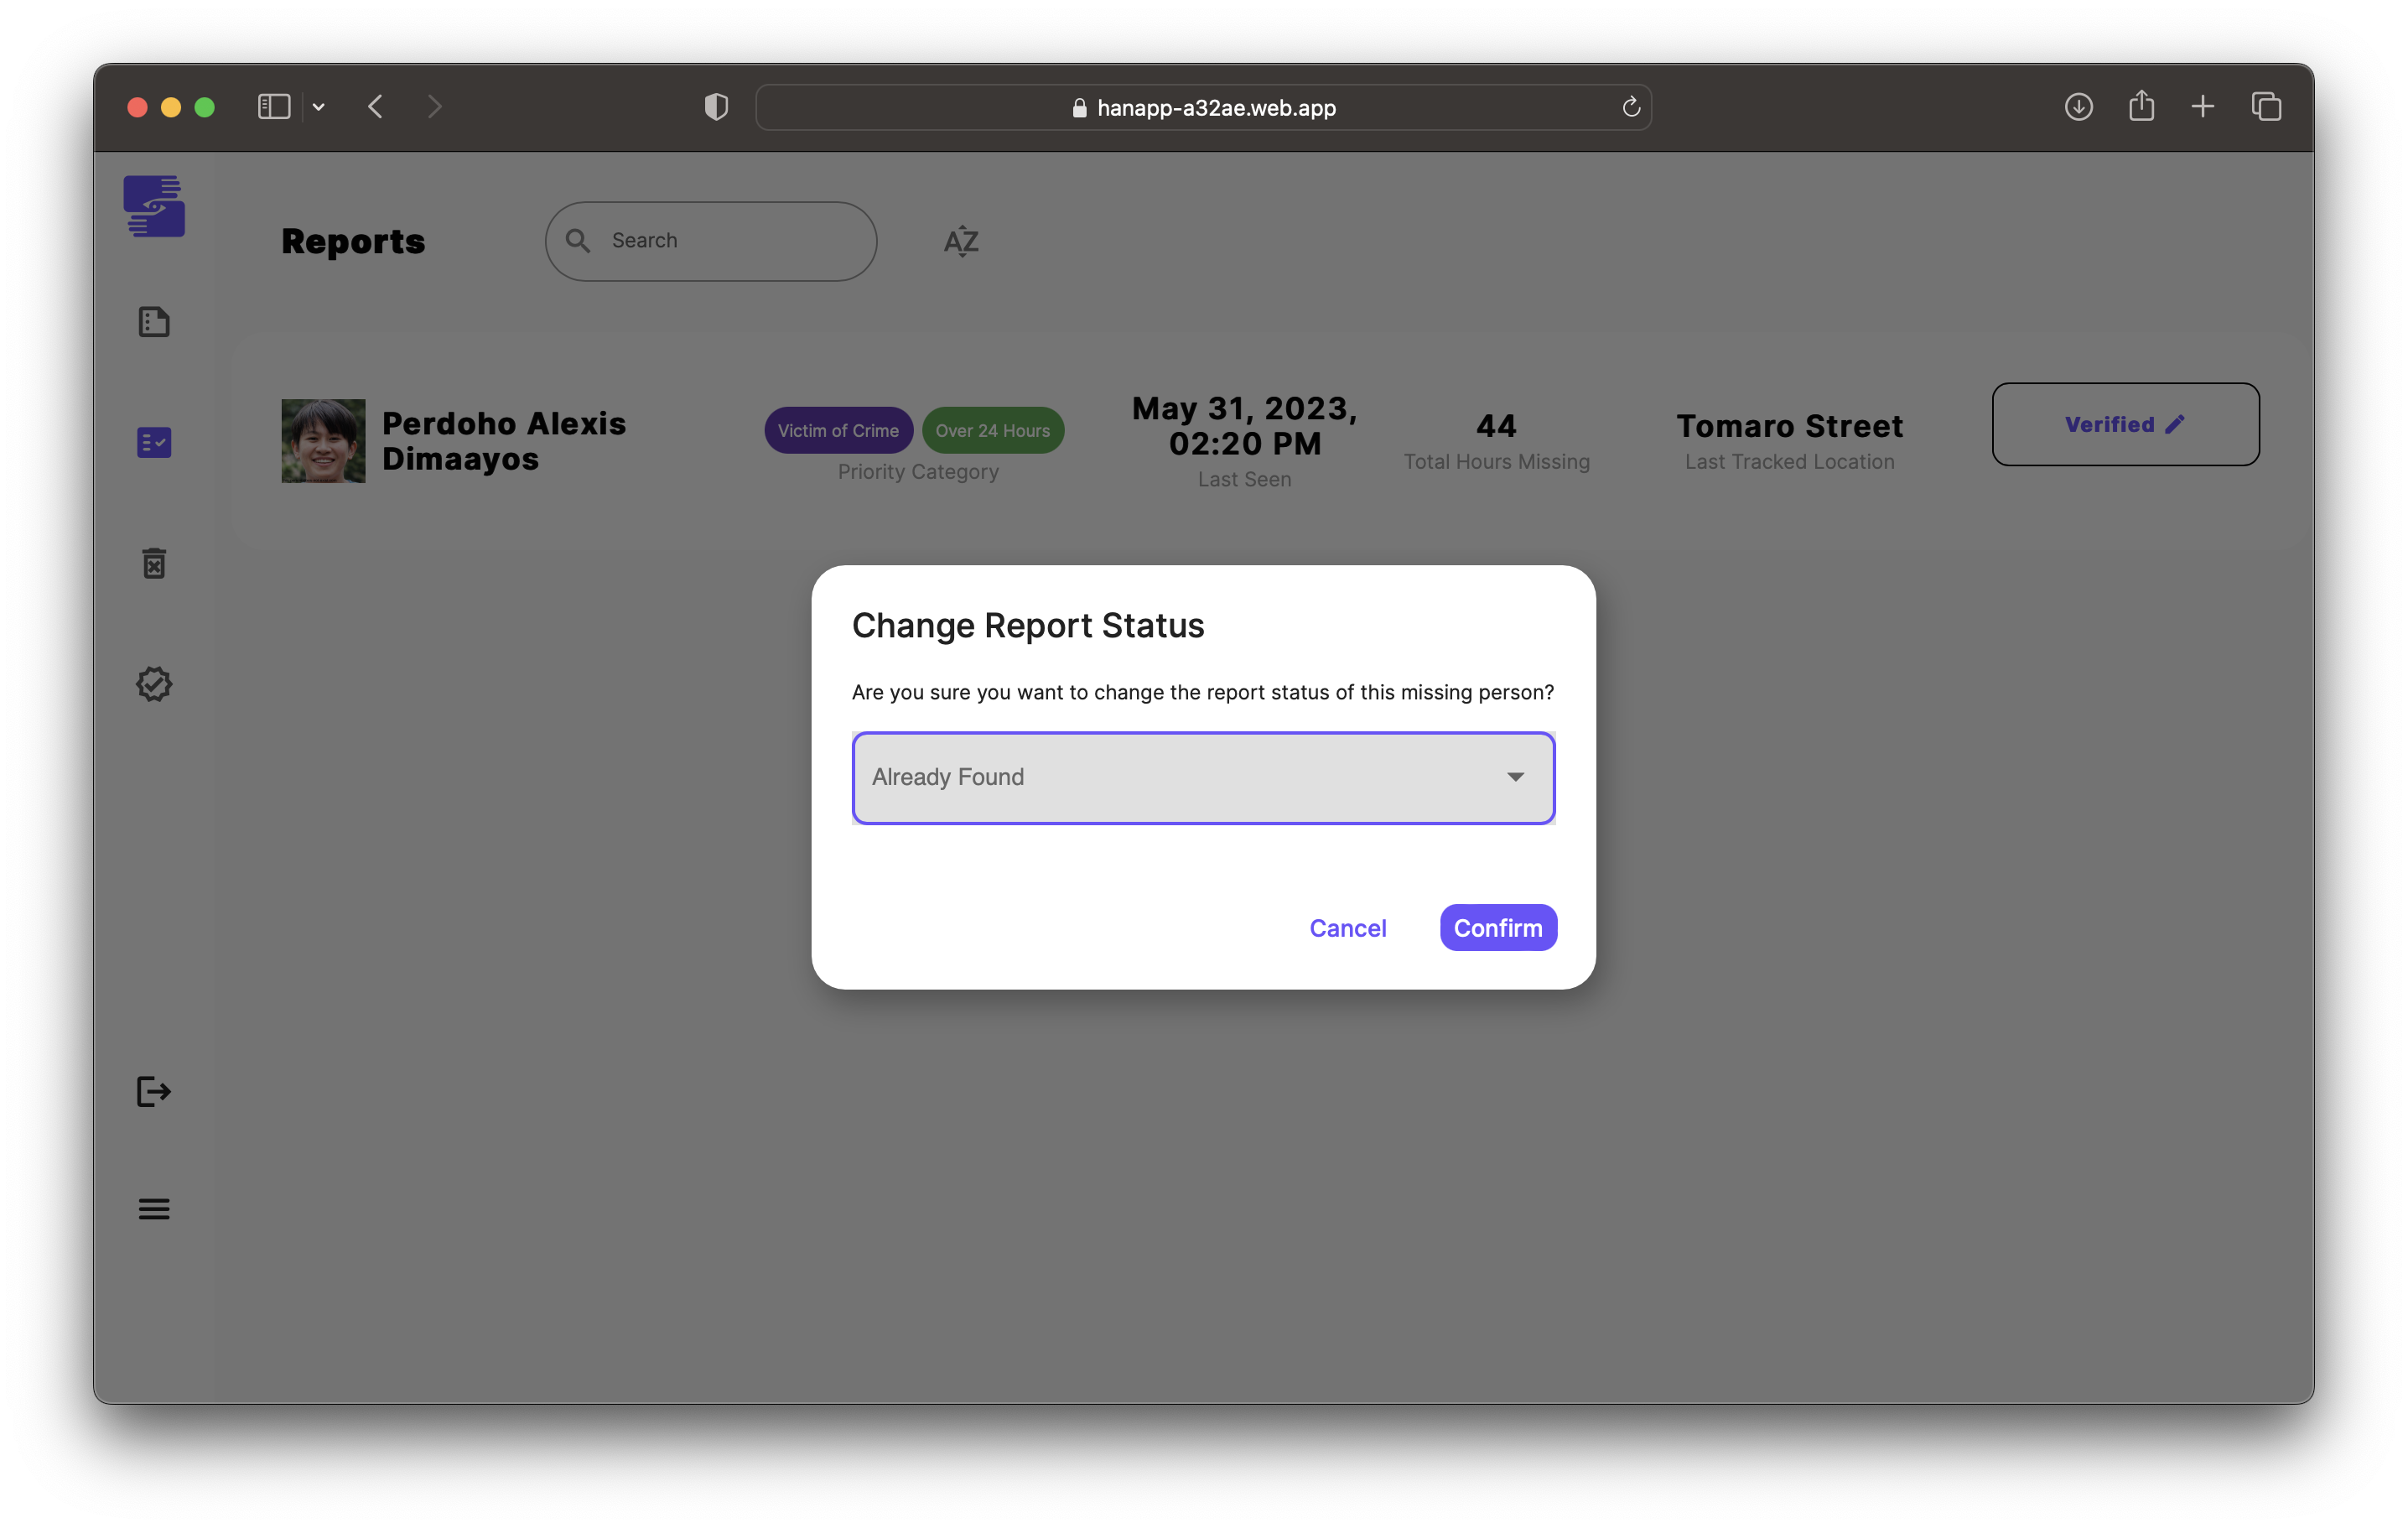
\includegraphics[scale=0.20]{figures/Chapter4/PNP/ChangeStatus-3.png}
    \end{subfigure}
    \centering
    \begin{subfigure}[c]{1\linewidth}
        \centering
        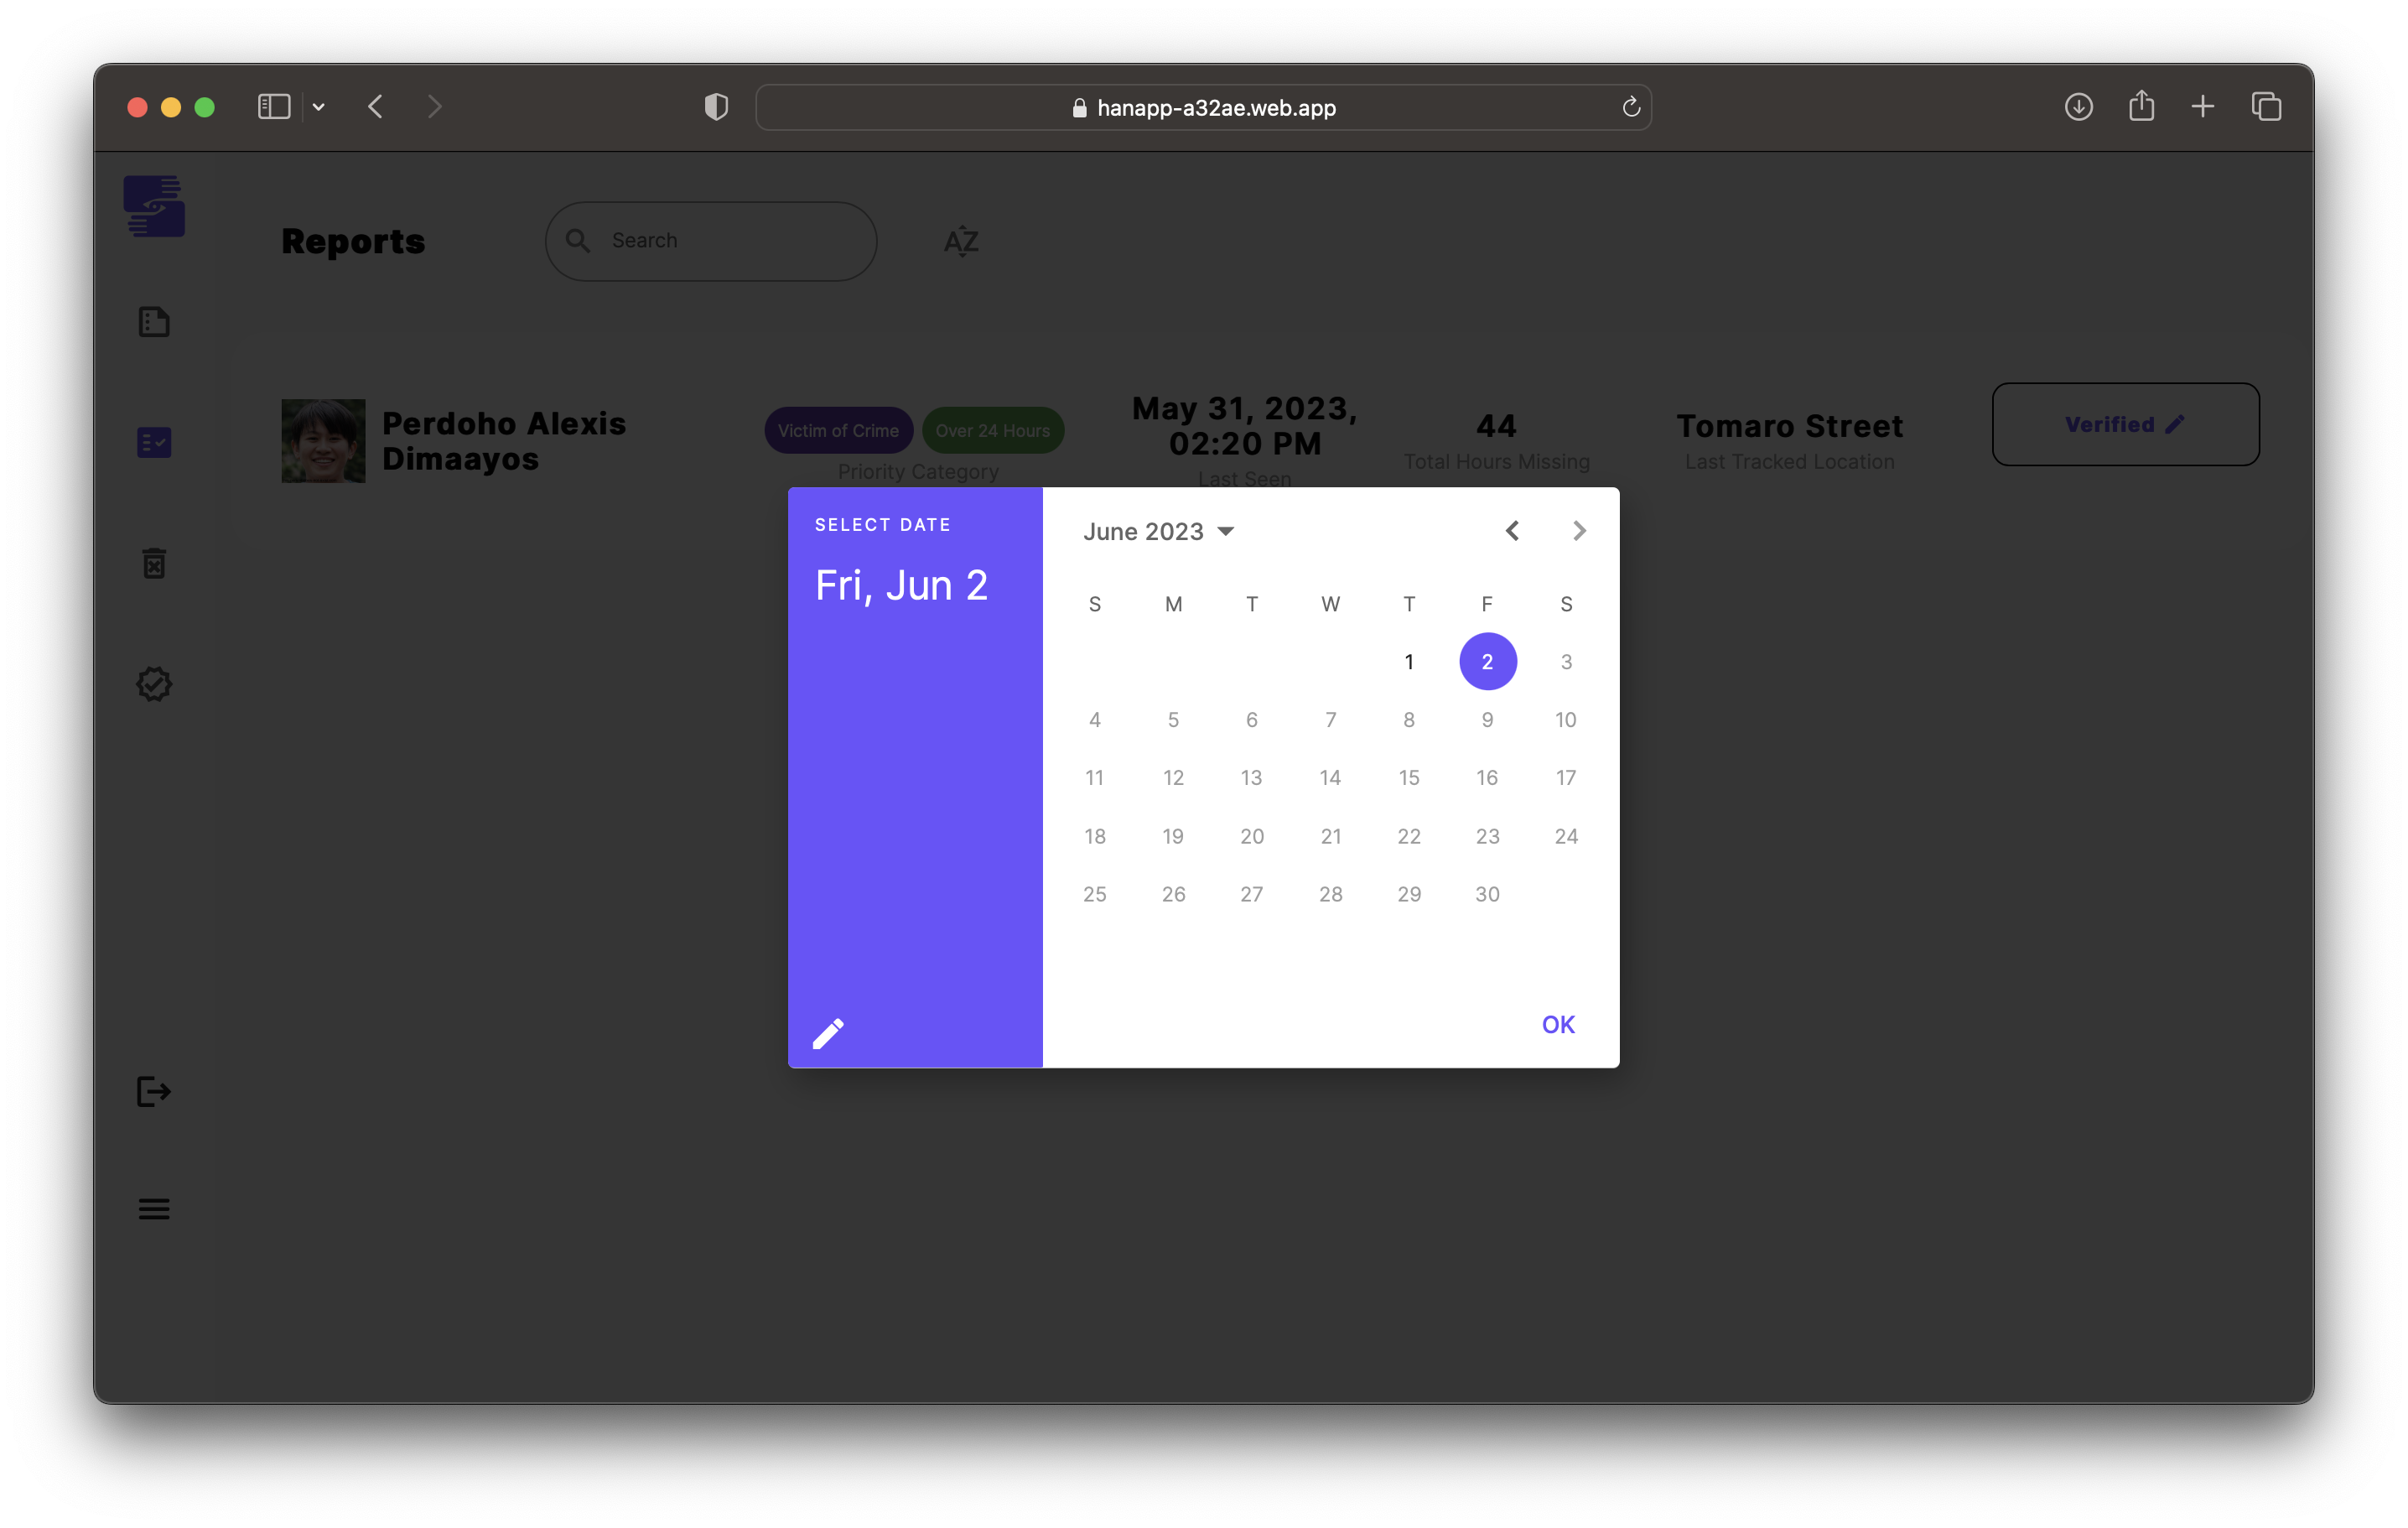
\includegraphics[scale=0.20]{figures/Chapter4/PNP/ChangeStatus-4.png}
    \end{subfigure}
    \centering
    \begin{subfigure}[c]{1\linewidth}
        \centering
        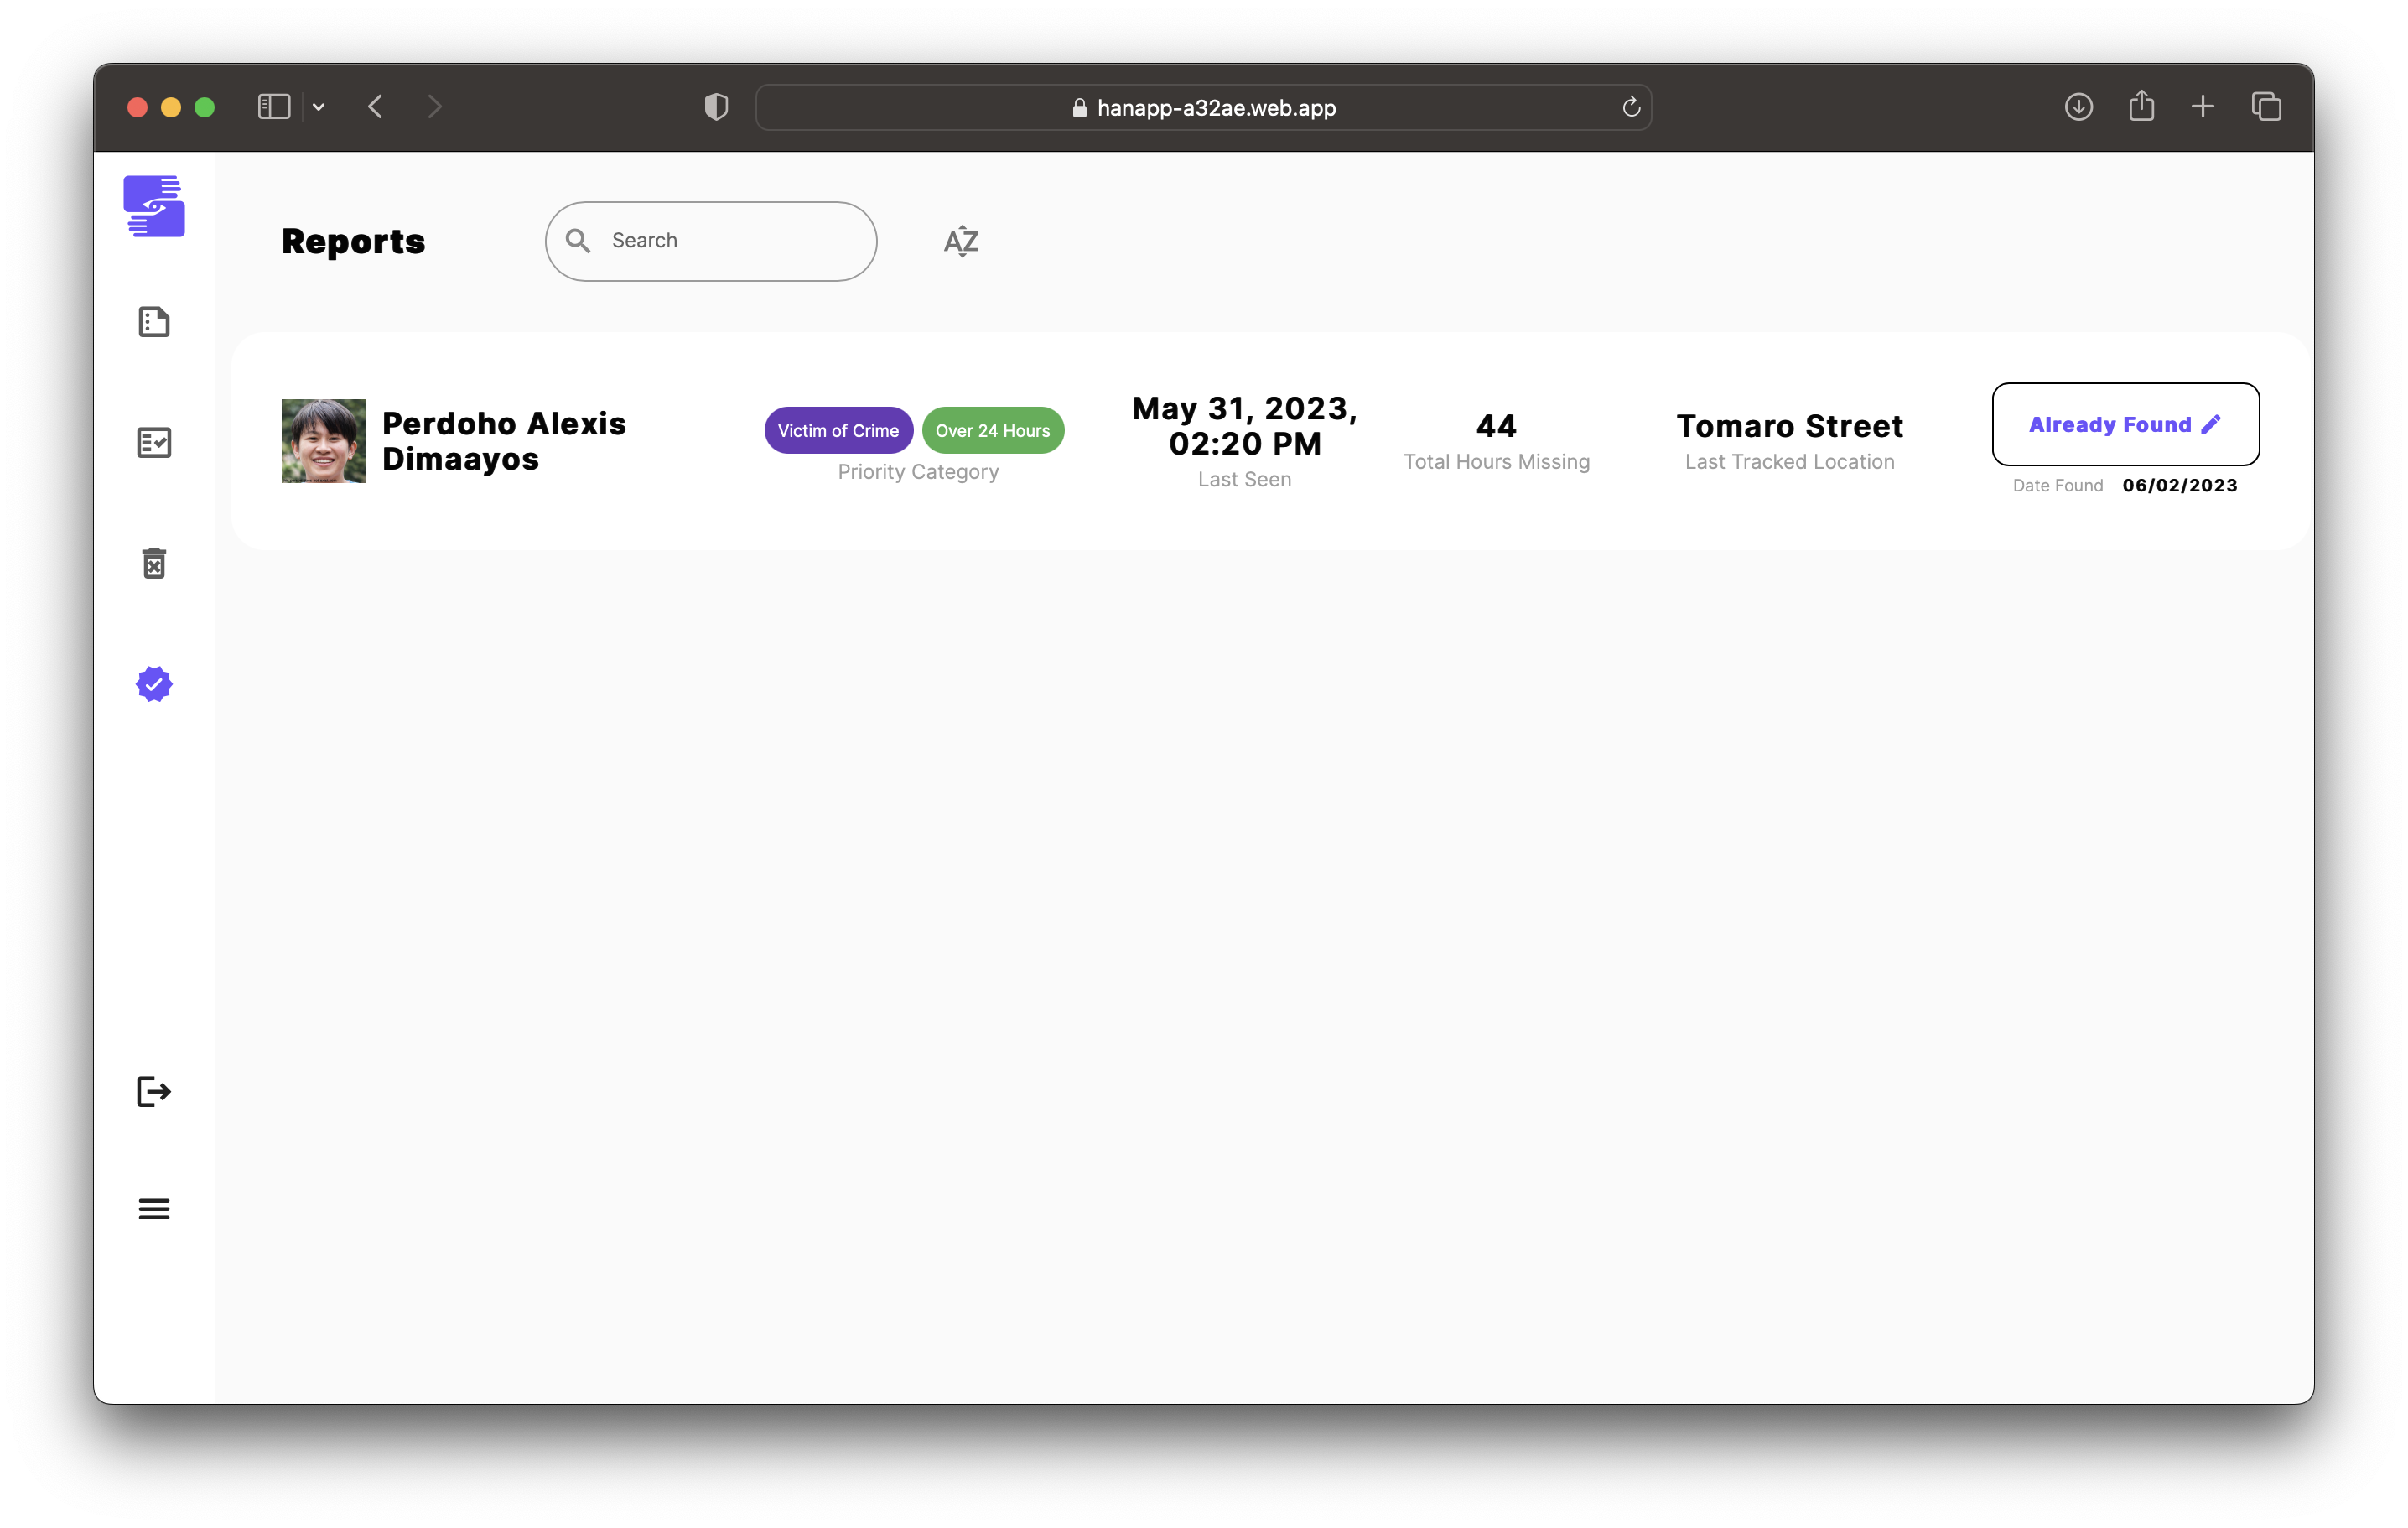
\includegraphics[scale=0.20]{figures/Chapter4/PNP/Already Found.png}
    \end{subfigure}
    \caption{Change Status to Already Found}
    \label{fig:ChangeStatusFound}
\end{figure}

\begin{figure}[!h]
    \centering
    \begin{subfigure}[c]{1\linewidth}
        \centering
        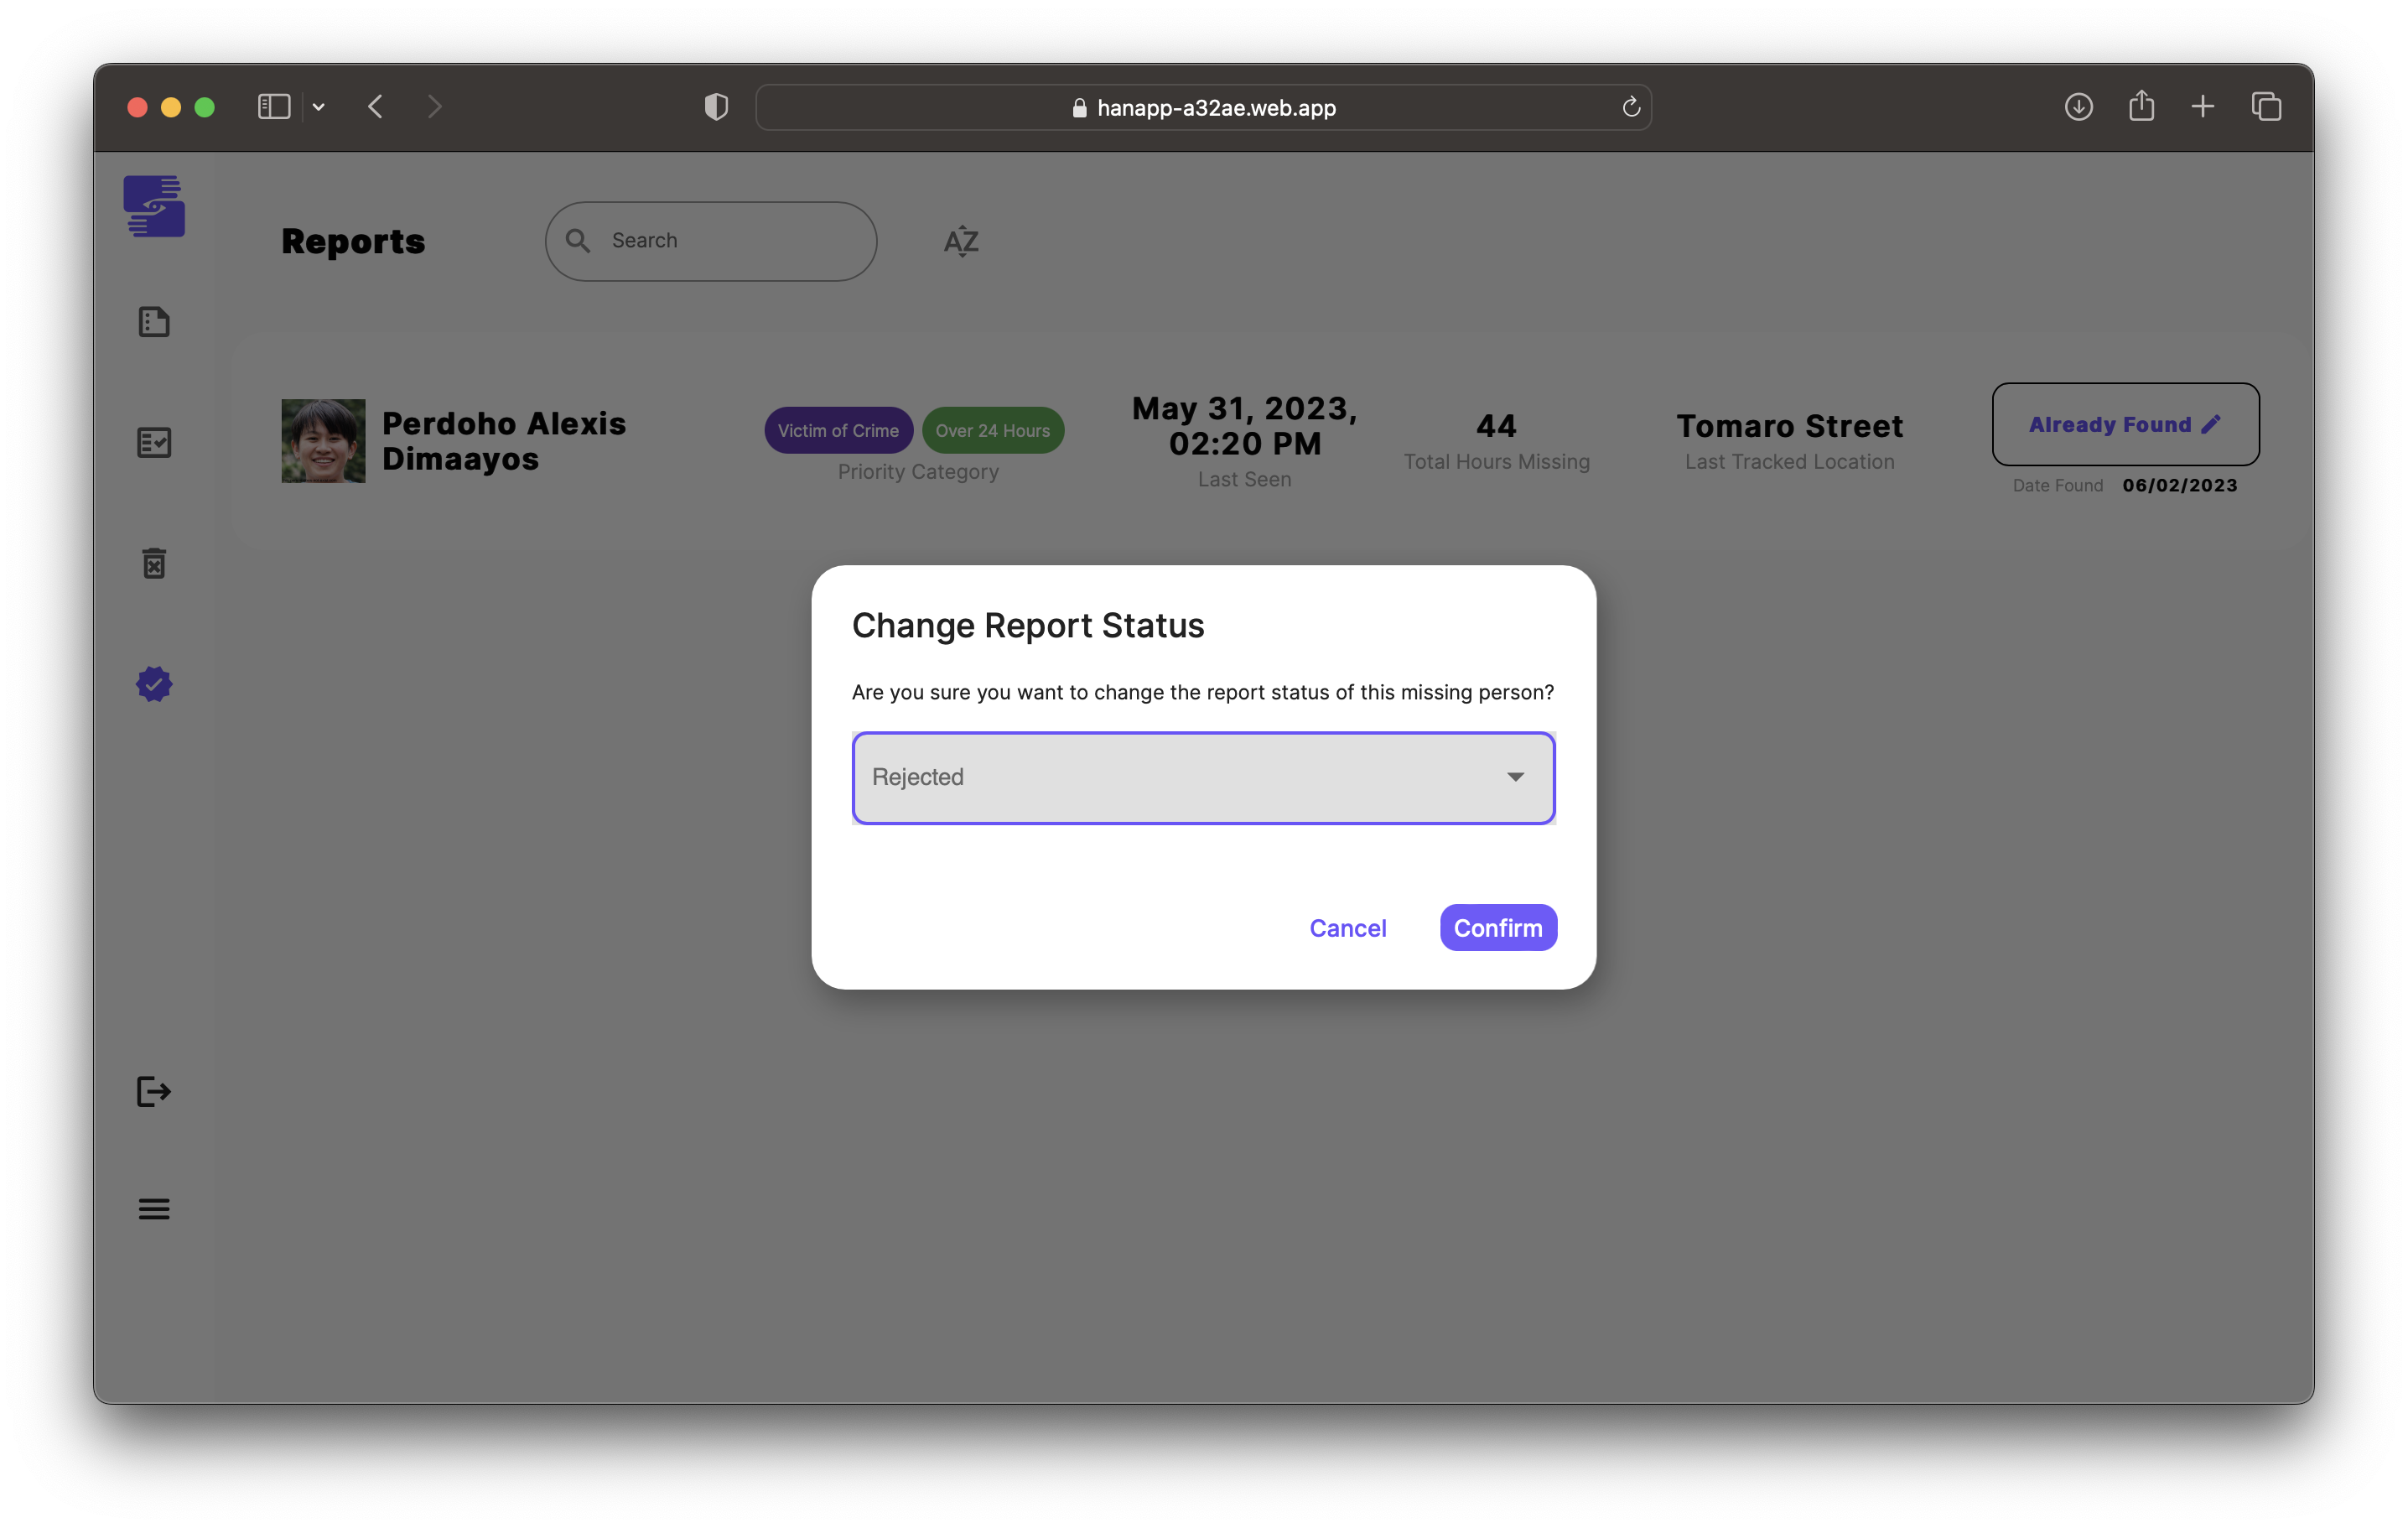
\includegraphics[scale=0.20]{figures/Chapter4/PNP/Rejected-1.png}
    \end{subfigure}
    \centering
    \begin{subfigure}[c]{1\linewidth}
        \centering
        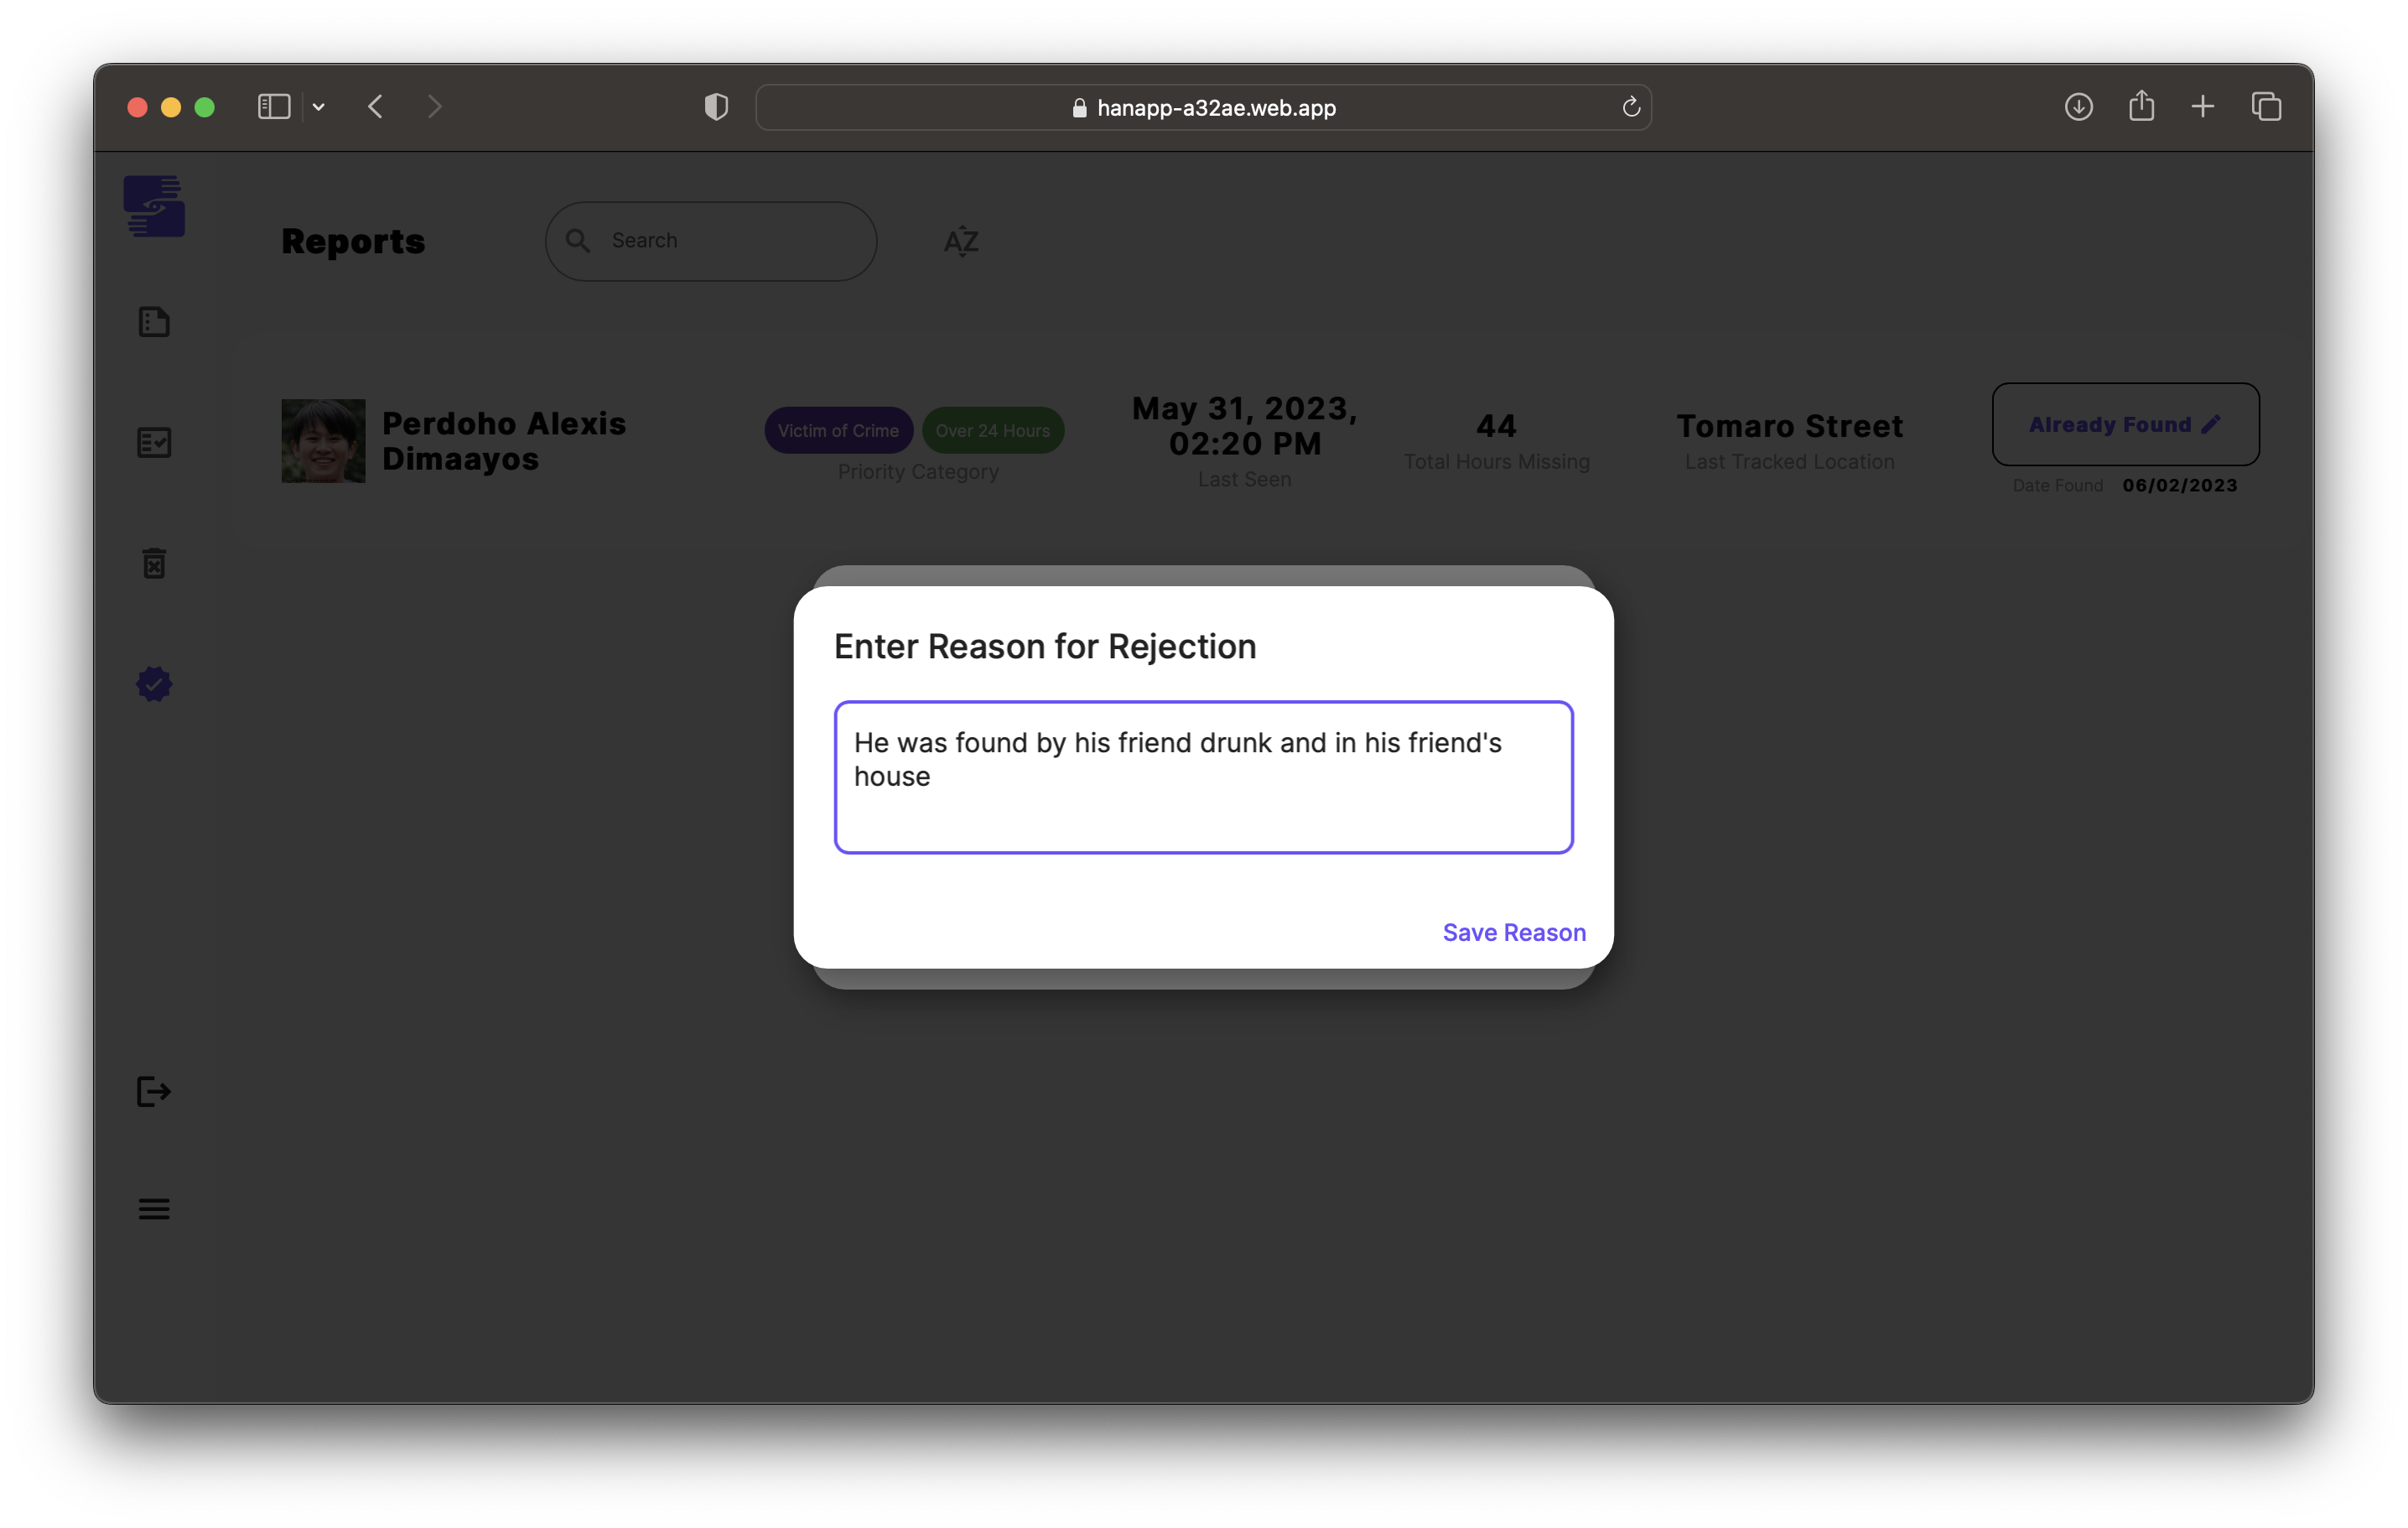
\includegraphics[scale=0.20]{figures/Chapter4/PNP/Rejected-2.png}
    \end{subfigure}
    \centering
    \begin{subfigure}[c]{1\linewidth}
        \centering
        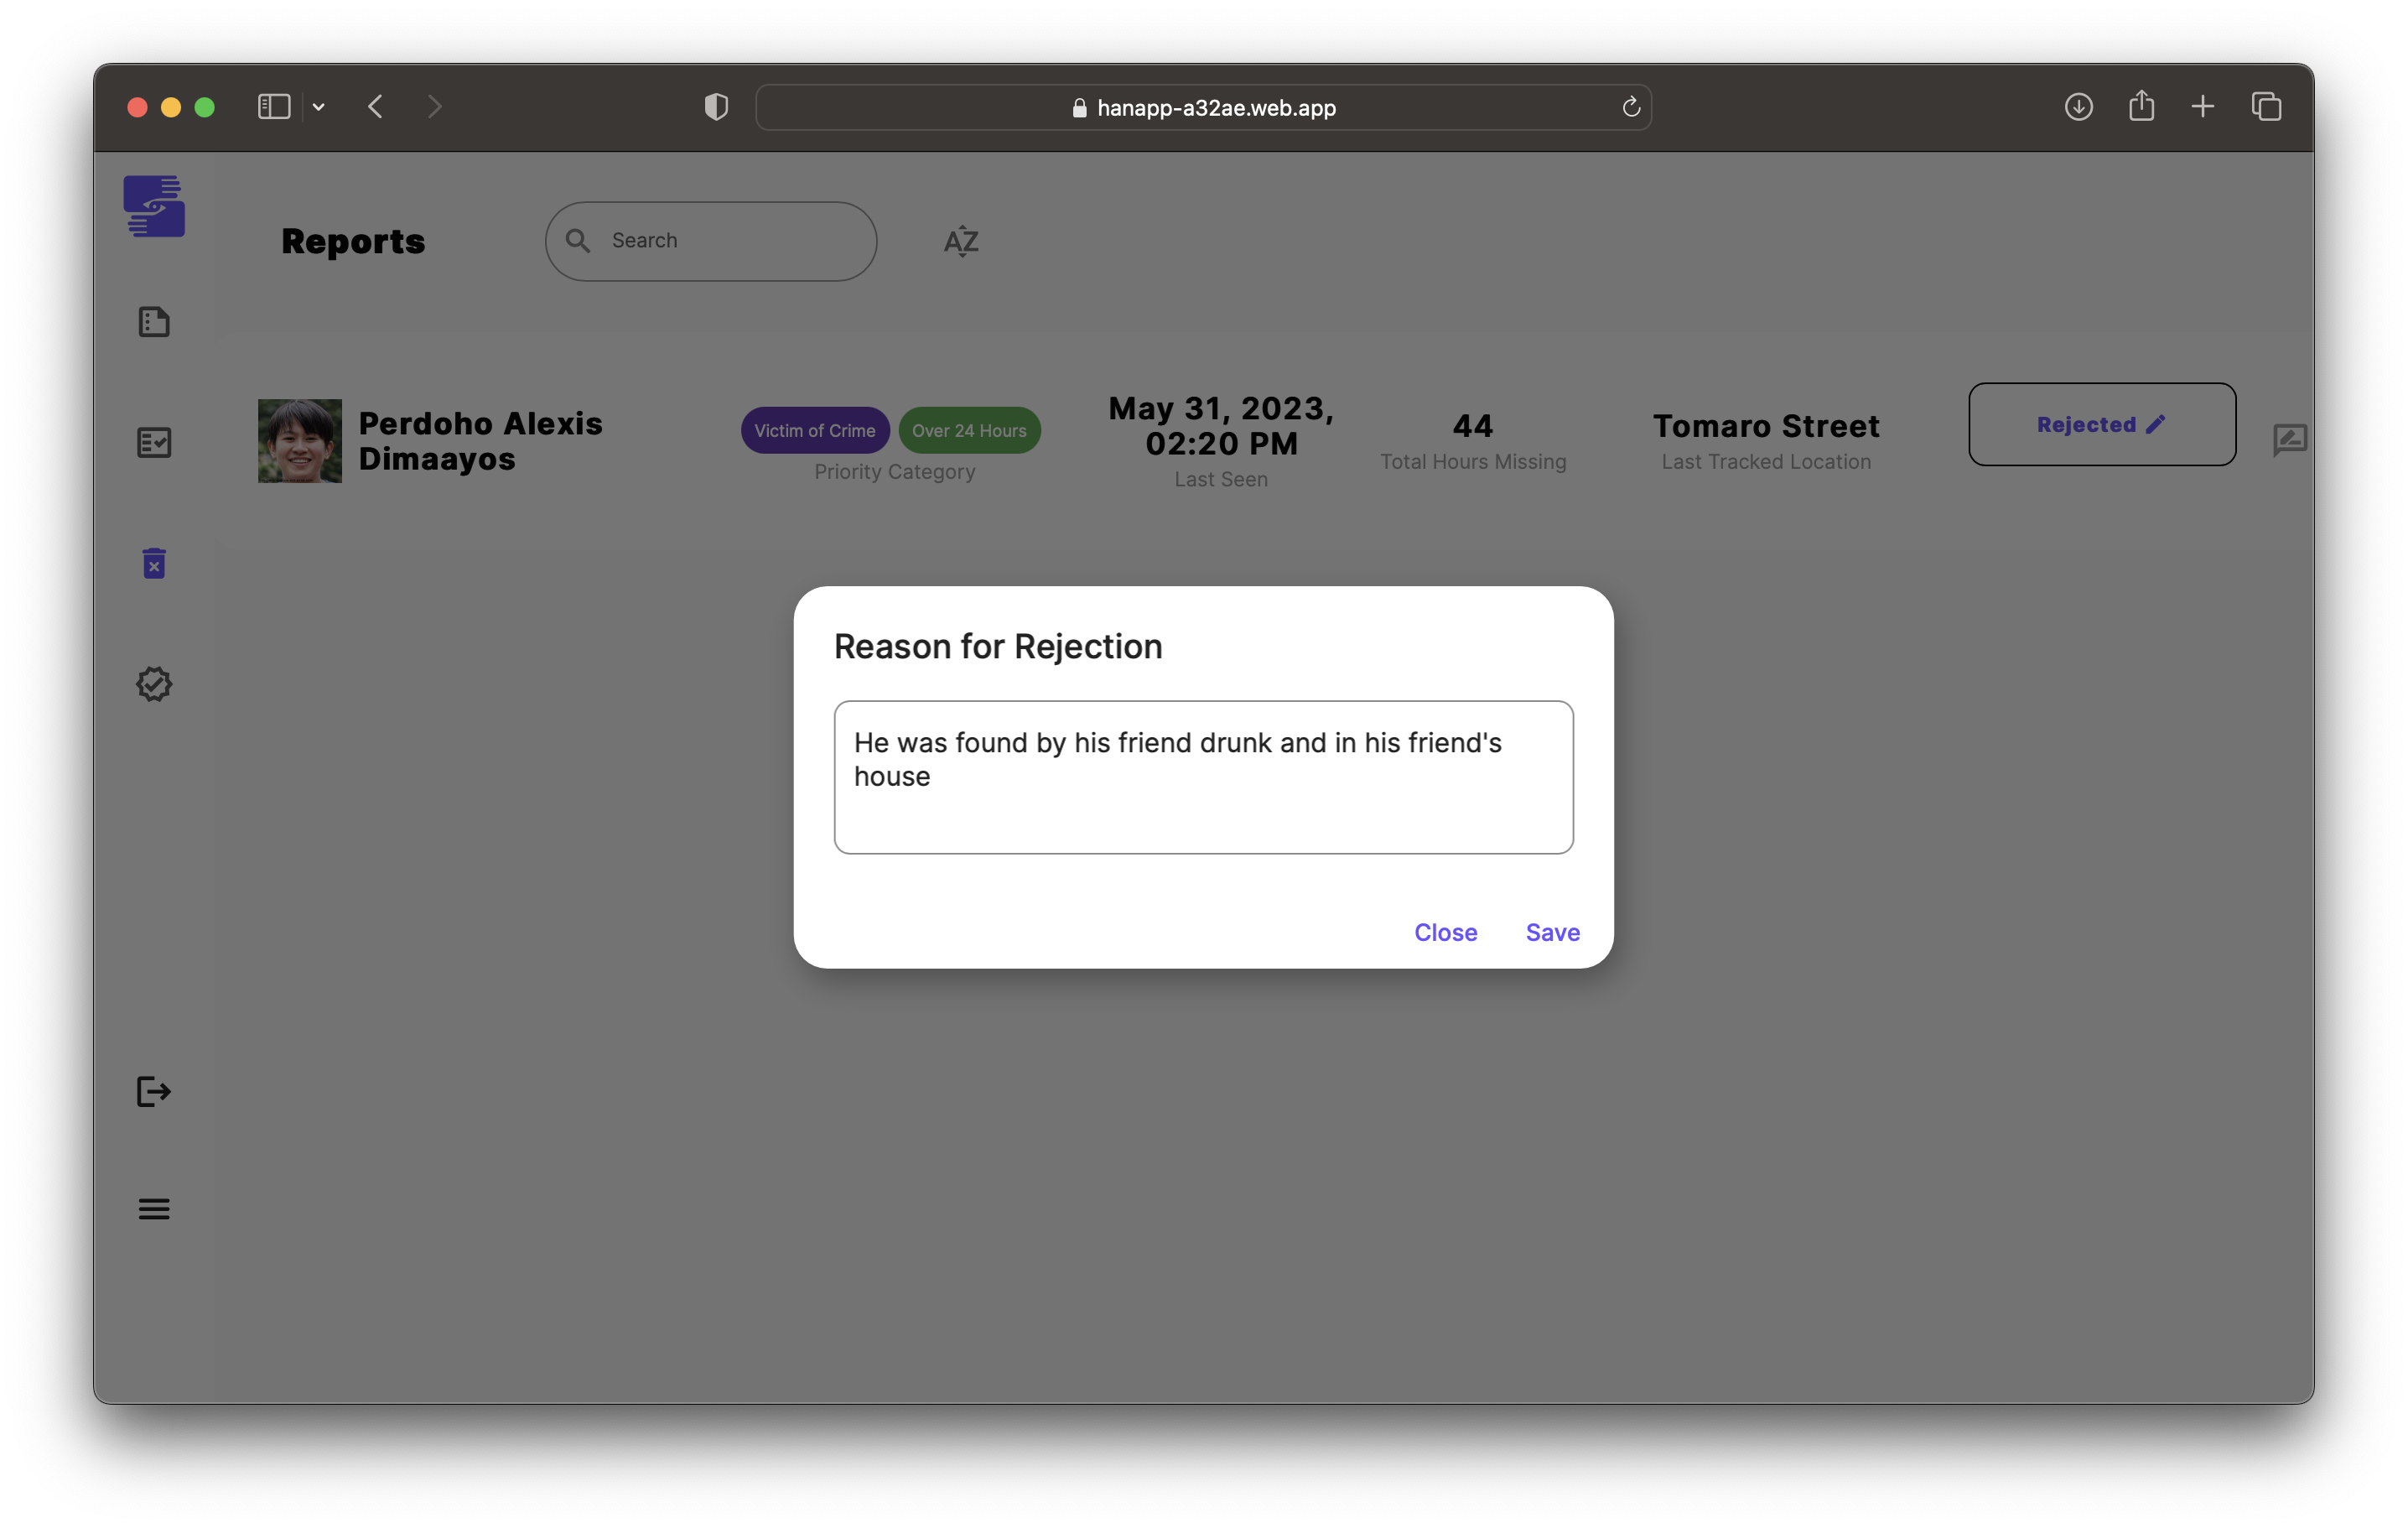
\includegraphics[scale=0.20]{figures/Chapter4/PNP/Rejected-4.png}
    \end{subfigure}
    \caption{Change Status to Rejected}
    \label{fig:ChangeStatusRejected}
\end{figure}

%
%  Indicate your resource persons here:
%
%	<full name and title, e.g., Dr. Juan de la Cruz>
%	<profession, e.g., faculty>
%	<department, e.g., Division of Physical Sciences and Mathematics>
%	<name of institution, e.g., University of the Philippines Visayas>
%	<e-mail address>
%
%

%
%  the following shows 3 examples, replace entries with your own
%

%\newcommand{\resperson}[4]{\textbf{#1} \\ #2 \\ #3 \\ \url{#4}\vspace{0.5em}\\}

%\resperson{Dr. Firstname1 Lastname1}{Adviser}{Affiliation1}{emailaddr@domain.com}
%\resperson{Mr. Firstname2 Lastname2}{Role2}{Affiliation2}{emailaddr2@domain.com}
%\resperson{Ms. Firstname3 Lastname3}{Role3}{Affiliation3}{emailaddr3@domain.net}